%% 
%% ACS project dissertation template. 
%% 
%% Currently designed for printing two-sided, but if you prefer to 
%% print single-sided just remove ",twoside,openright" from the 
%% \documentclass[] line below. 
%%
%%
%%   SMH, May 2010. 


\documentclass[a4paper,12pt,twoside,openright]{report}


%%
%% EDIT THE BELOW TO CUSTOMIZE
%%

\def\authorname{Alexander\ Harri\ Bell-Thomas\xspace}
\def\authorcollege{Jesus College\xspace}
\def\authoremail{Alexander.Bell-Thomas@cl.cam.ac.uk}
\def\dissertationtitle{Trusted Reference Monitors for Linux using Intel SGX Enclaves}
\def\wordcount{14,235}


%\usepackage[dvips]{epsfig,graphics} 
\usepackage{epsfig,graphicx,verbatim,parskip,tabularx,setspace,xspace,geometry}
\usepackage{libertine}

%% START OF DOCUMENT
\begin{document}


%% FRONTMATTER (TITLE PAGE, DECLARATION, ABSTRACT, ETC) 
\pagestyle{empty}
\singlespacing
\newgeometry{margin=1.4in}
% title page information
\begin{titlepage} 

\begin{center}
\vspace*{1mm}
\noindent
\huge
\dissertationtitle \\
\vspace*{\stretch{1}}
\end{center}

\begin{center}
\noindent
\LARGE
\authorname \\
\Large
\authorcollege      \\[34pt]
%\begin{figure}

\includegraphics[width=0.42\textwidth]{figures/cambridge.eps}
%\end{figure}
\end{center}

\vspace{24pt} 

\begin{center}
\noindent
\large
{\it A dissertation submitted to the University of Cambridge \\ 
in partial fulfilment of the requirements for the degree of \\ 
Master of Engineering in Computer Science} 
\vspace*{\stretch{1}}
\end{center}

\begin{center}
\noindent
University of Cambridge \\
Computer Laboratory     \\
William Gates Building  \\
15 JJ Thomson Avenue    \\
Cambridge CB3 0FD       \\
{\sc United Kingdom}    \\
\end{center}

\begin{center}
\noindent
Email: \authoremail \\
\end{center}

\begin{center}
\noindent
\today
\end{center}

\end{titlepage} 

\newpage
\vspace*{\fill}

\restoregeometry
\onehalfspacing
\newpage
{\Huge \bf Declaration}

\vspace{24pt} 

I, \authorname of \authorcollege, being a candidate the Part III of
the Computer Science Tripos, hereby declare that this report and the
work described in it are my own work, unaided except as may be
specified below, and that the report does not contain material that
has already been used to any substantial extent for a comparable
purpose.

\vspace{24pt}
Total word count: \wordcount

\vspace{60pt}
\textbf{Signed}: \textit{A.H. Bell-Thomas}

\vspace{12pt}
\textbf{Date}: \textit{\today}


\vfill

This dissertation is copyright \copyright{} 2020 \authorname. 
\\
All trademarks used in this dissertation are hereby acknowledged.



\newpage
\vspace*{\fill}

\singlespacing
\newpage

\ifblind 

\begin{center}
    \vspace*{1mm}
    \noindent
    \huge
    \dissertationtitle \\
    % \vspace*{\stretch{1}}
    \vspace{18pt} 
    {\large \bf \sc Abstract}
    \vspace{12pt} 
\end{center}

\else
{\Huge \bf Abstract}
\vspace{24pt} 
\fi


\paragraph{} Information Flow Control (IFC) is a powerful tool for protecting data in a computer system, enforcing not only who may access it, but also how it may be used throughout its lifespan. Intel's Software Guard Extension (SGX) affords complementary protection, providing a general-purpose Trusted Execution Environment for applications and their data. To date, no work has been conducted considering the overlap between the two, and how they may mutually reinforce each other.

\paragraph{} This dissertation presents \textsc{Citadel}, a modular, SGX-backed reference monitor to securely and verifiably implement IFC methods in the Linux kernel. Its prototype externalises policy decisions from its enforcement security module, providing a userspace promise-of-access model with asynchronous fulfillment. By aliasing system calls, the system transparently integrates with unmodified applications, and amortises the performance cost of integration by inferring processes' underlying security contexts.

\paragraph{} Observed results are promising, demonstrating a worst-case median performance overhead of $25\%$. In addition, the \textsc{Nginx} webserver is demonstrated running under \textsc{Citadel}; high bandwidth transfers exhibit near parity with the native Linux kernel's performance. This work illustrates the potential viability of a symbiotic enclave-kernel relationship for security implementations, something that may, in the long run, benefit both.



\newpage

\vspace*{\fill}


\pagenumbering{roman}
\setcounter{page}{0}
\pagestyle{plain}
\tableofcontents
\listoffigures
\listoftables

\onehalfspacing

%% START OF MAIN TEXT 

\chapter{Introduction}
\pagenumbering{arabic} 
\setcounter{page}{1} 
\paragraph{} This is my introduction

\chapter{Background} 

\paragraph{} This chapter will cover a number of topics essential to understanding the rationale and implementation of the design as discussed in §~\ref{sec:design}. These include; an introduction to \textit{Information Flow Control} (\textit{IFC}), the Intel SGX platform, and an overview of key aspects of the Linux kernel relevant to the architecture of the prototype.


% -------------

\section{Information Flow Control}
\label{sec:ifc}

\paragraph{} IFC regulates how and where data is permitted to move and be transformed in a computer system.~\cite{ifc-data-prop} This differs from access control, which defines \textit{what} resources may be used by an entity --- IFC allows granular control over \textit{how} they may be used once accessed, including restricting propagation between components. 

\paragraph{} Formally, IFC defines and enforces a non-interference policy between abstract \textit{security contexts}. A simple, atomic example is the distinction between \textit{unclassified} and \textit{classified} data --- here, information is only allowed to flow \textit{up}, ensuring that an \textit{unclassified} entity does not learn anything marked as \textit{classified}.~\cite{Bell1973SecureCS} In general this form of relationship can be represented as a partial ordering over \textit{security contexts}, formulated as a lattice.~\cite{ifc-lattice}

\paragraph{} However, practical systems often require dataflow adhering to a more complicated policy set --- for example, supporting \textit{declassification}.~\cite{10.5555/794199.795122} Work undertaken by Pasquier et al.,~\cite{camflow} which will be the core influence of the IFC model developed in this project, constructs a pliable and efficient \textit{decentralised information flow control} (\textit{DIFC}) model suitable for provenance enforcement and auditing in the Linux kernel.

\paragraph{} The concepts presented are primarily derived from Pasquier~\cite{camflow} and Krohn et al.~\cite{flume}.

\subsection{Motivation, History, and \textit{Decentralised IFC}}

\paragraph{} IFC has, in recent years, been increasing in support as a powerful methodology for ensuring granularly privacy whilst simultaneously not unduly restricting access to sensitive information. IFC annotates data records with opaque \textit{labels} that refer to either their confidentiality or integrity status. Rather than simply restricting access to sensitive data, as would be the action taken by an access control mechanism, IFC opts to track data as it propagates --- if an entity attempts to move this into an unknown, untrusted, or conflicting \textit{security context} the IFC system prevents this to ensure data is not improperly released.

\paragraph{} IFC originated from research conducted in the mid-1970s~\cite{ifc-lattice} but has not, as of yet, seen mainstream adoption. A major reason for this is that early schemes were designed around the \textit{multi-level security} (\textit{MLS}) doctrine set out in the \textit{Orange Book}:~\cite{orange-book} this locked IFC to a shallow set of broad labels, mirroring existing institutional segregation (such as \textit{restricted}, \textit{secret}, \textit{top secret}). Policies were managed centrally, something easily applicable in settings with rigorous hierarchies such as the military, but unwieldy in an organisation with manifold security protocols.

\paragraph{} The majority of recent research in this area has advocated \textit{decentralised information flow control} 
(\textit{DIFC}), introduced by Myers and Liskov.~\cite{difc,10.1145/363516.363526,10.1145/268998.266669} DIFC is more granular that schemes adhering to the \textit{MLS} model, for example, creating two distinct \textit{security contexts} for two files in the same folder. Policies are \textit{discretionary}, allowing users to specify and modify the enforced policies for assets they own.

\subsection{Security Labels and the Reference Monitor}

\paragraph{} A DIFC system relies on \textit{tags} and \textit{labels} to annotate the entities it tracks. Let $\mathcal{T}$ be a large set of opaque tokens, or \textit{tags}. An individual tag does not carry any particular meaning by itself, but is used as an abstract identifier for the integrity or secrecy of an entity's \textit{security context}. A \textit{label}, $l \subseteq \mathcal{T}$, is a collection of tags that are concretely attached to assets, such as files; these form a lattice under the subset-relation partial order. For each process $a$ there are two labels, one for secrecy, $a_s$, and one for integrity, $a_i$. For a tag $t$, $t \in a_s$ implies, conservatively, that process $a$ has seen information associated with tag $t$. Likewise, $t \in a_i$ indicates that every input to $a$ has been endorsed for an integrity level marked with $t$.

\paragraph{Walkthrough --- Secrecy Enforcement} In a typical environment, a user can only convince themselves that a text editor is safe to use it they, or someone they trust, audits the program's source code. With DIFC however, it is possible to reason that if the system can provide the following four guarantees, it cannot leak sensitive data without the user's permission.

\begin{enumerate}
    \item If a process $a$ read a file with a secrecy tag $t$, then $t \in a_s$.
    \item $t \in a_s$ implies that $a$ cannot communicate with another process, $b$, where $t \notin b_s$.
    \item $a$ cannot remove $t$ from $a_s$ without permission.
    \item $t \in a_s$ restricts $a$'s access to an uncontrolled medium, such as a network.
\end{enumerate}

\paragraph{} The heart of an IFC implementation is its \textit{Reference Monitor}, which tracks the labelling for each process, granting or rejecting permission to execute an operation before being served to the operating system. Different solutions handle this process differently: \textit{Flume},~\cite{flume} for example, implements a full system interposition layer, forcing all \textit{syscalls} to pass through its userspace \textit{reference monitor} before reaching the OS, whereas \textit{CamFlow}~\cite{camflow} embeds its \textit{reference monitor} in the kernel itself. In all schemes, however, this trusted component is responsible for the policy and its enforcement on the system. This project focusses on this implementation.


\subsection{Modelling}
\label{sec:ifc-modelling}

\begin{table}
    \centering
    \newcommand\tableTop{\rule{0pt}{3ex}}
    \newcommand\tableMid{\rule{0pt}{3ex}}
    \newcommand\tableBottom{\rule[-2ex]{0pt}{0pt}}
    \begin{tabular}{r p{10cm}} 
        \hline
        Notation & Explanation \\ [0.1ex] 
        \hline
            \tableTop{$A \rightarrow B$} & \tableTop{Rule $\alpha$; a permissible information flow between entity $A$ and entity $B$.} \\
            
            $A \Rightarrow B$ & \tableMid{Rule $\beta$; a creation flow, initialising $B$ from $A$ as its parent.} \\

            $A \rightsquigarrow A'$ & \tableMid{Rule $\gamma$; a context change, with $A$ modifying its security context in accordance with its capabilities.} \\
            
            $A \xhookrightarrow[]{t^{\pm}_{x}} B$ & \tableMid{Rule $\delta$; priviledge delegation, with $A$ passing a capability $t_{x}^{\pm}$ to $B$.} \tableBottom \\
    \end{tabular}
    % \vspace{5mm}
    \caption{Overview of the four core IFC events used in §~\ref{sec:ifc-modelling}.}
    \label{table:ifc-notation}
\end{table}


\paragraph{} In centralised IFC schemes, the reference monitor is the only entity capable of creating, changing, and assigning tags. DIFC modifies this, giving \textit{all} processes the ability to create and modify tags for entities they hold ownership over; thus they alone have the right to declassify them.

\paragraph{Notation} As the model we build in §~\ref{sec:design} is closest in spirit to \textit{CamFlow}, we, for clarity in comparison, use the same notation (as summarised in Table~\ref{table:ifc-notation}).

\paragraph{Enforcing Safe Flows} ($\alpha$), below, describes the conditions in which a flow can be considered \textit{safe}, abiding by the system's IFC policy. Verbally, the recipient must be \textit{at least as privileged} as the originator and cannot accept information graded below its own integrity status. Here $\preceq$ denote any applicable preorder relation; this context uses inclusion ($\subseteq$). If a flow is \textit{impermissible} it is denoted as $A \nrightarrow B$.
\begin{equation}
    A \rightarrow B \iff A_s \preceq B_s \;\; \land \;\; B_i \preceq A_i \tag{$\alpha$}
\end{equation}
\paragraph{} Information produced within a \textit{security context} may only flow within the same context or a related \textit{subcontext}. Integrity functions in the same way but in the inverse; data can only flow in contexts with the same, or lower, integrity grading.

\paragraph{Entity Creation} Correct initialisation of a new object's \textit{security context} is shown in ($\beta$). Logically it must be held at the same level as the environment creating it. An illustrative example is a process creating a new file; although permitted the result is subject to the same tainting as the original process.
\begin{equation}
    A \Rightarrow B \implies A_s = B_s \;\; \land \;\; A_i = B_i \tag{$\beta$}
\end{equation}

\paragraph{Vocational Label Management} The core mantra of the \textit{decentralised} aspect of \textit{DIFC} is that processes are themselves responsible for policies governing the assets they own. To this end, a process's labelling must be dynamic. Generally, entities can be sorted into two distinct categories;

\begin{itemize}
    \item \textit{Active} (processes), with \textit{mutable} security contexts.
    \item \textit{Passive} (files, pipes, sockets, etc.), which merely act as data vessels for \textit{active} entities.
\end{itemize}

\paragraph{} \textit{Active} entities have the right to modify their labelling iff they have the capability to make that modification. These capabilities come in two forms; one for addition and one for removal of tags. The set $A_{s}^{+} \subseteq \mathcal{T}$ enumerates all the tags that entity $A$ has the ability to add to its security labelling. Likewise, $A_{s}^{-} \subseteq \mathcal{T}$ holds all of the tags $A$ has the ability to remove from its labelling. These sets are modified either in the process of creating an entity or in receipt of a delegated capability from a peer. The sets $A_{i}^{\pm} \subseteq \mathcal{T}$ also exist, performing the same function for integrity labels. ($\gamma$) describes this process formally.
\begin{equation}
    \left\{\begin{array}{lr}
        A'_x \leftarrow A_x \cup \{t\} & \text{if} \;\; t \in A_{x}^{+} \\
        A'_x \leftarrow A_x \smallsetminus \{t\} & \text{if} \;\; t \in A_{x}^{-} \\
    \end{array}\right\} \implies A \rightsquigarrow A' \tag{$\gamma$}
\end{equation}

\paragraph{} A notable restriction is that a process has to be aware of the IFC constraints imposed on it and how to interact with the system to perform this operation. Most processes should not require this, but is an important consideration when applying DIFC to an entire system.

\paragraph{Capability Lifecycle and Delegation} As defined by ($\beta$), an entity automatically inherits the labelling of its creator: this process, however, does not pass on any capabilities ($A_{s}^{\pm}, A_{i}^{\pm} = \varnothing$). This raises the need for \textit{capability delegation}.

\paragraph{} A capability held by $A$, $t_{x}^{\pm}$, where $t \in A_{x}^{\pm}$, is permitted to be transferred to $B$ in order for it to act on its behalf. Delegation is denoted as follows in ($\delta$).


\begin{equation}
    A \xhookrightarrow[]{t^{\pm}_{x}} B \;\; \text{only if} \;\; t \in A_{x}^{\pm} \tag{$\delta$}
\end{equation}

\paragraph{} As an example, delegation is vital for a web server. To transmit another entity's information over an untrusted socket the server must have permission to \textit{declassify} it --- i.e. it must hold $f_{s}^{-}$, where $f$ is the secrecy label of the information to transmit.\footnote{The server process, $W$, must have $W_{i} = \varnothing$ as it holds a connection to an untrusted socket. Thus the integrity clause in ($\alpha$) will not interfere.}


% ---------

\section{Intel® SGX}

\paragraph{} Intel's Software Guard Extensions, SGX, was first announced and detailed in a handful of whitepaper documents published from 2013.~\cite{10.1145/2487726.2488370, 10.1145/2487726.2488368, Anati2013InnovativeTF, sgx-sgx-reference} It described a novel approach to \textit{trusted computing}, creating in-CPU containers with dedicated protected memory pools. These regions, called \textit{enclaves}, cannot be read from or written to by an unauthorised party due to fundamental protection mechanisms provided by the x86 architecture, even if running in \textit{Ring 0}:\footnote{x86 offers four protection \textit{rings}, of which Linux uses two --- \textit{0} for the kernel, and \textit{3} for userspace.} Figure~\ref{fig:sgx-basic} illustrates this. \textit{Enclaves} guarantee both integrity and secrecy to the application running inside it, even in the presence of a malicious host.

\paragraph{Motivation} At a high-level SGX aims to achieve security for sensitive applications by shielding them, and the resources they use, against tampering, and to provide a guarantee to end-users of an enclave's integrity; this is achieved using attestation and measurement (described in §~\ref{sec:attestation}). One of many use cases~\cite{10.1145/2834050.2834100, 10.1145/2799647, 10.1145/2810103.2813695} is in a cloud computing context, where users are forced to trust an outside party with both their data and business logic. By distributing encrypted, yet executable, containers targetted at a single, unique SGX core, users can be assured that their information is safe, regardless of any virtualisation that may be taking place. Only the provisioned CPU is able to decrypt and execute the enclave, strictly in accordance with the restrictions of the SGX platform.

\subsection{Security Characteristics}

\begin{figure}[]
    \centering
    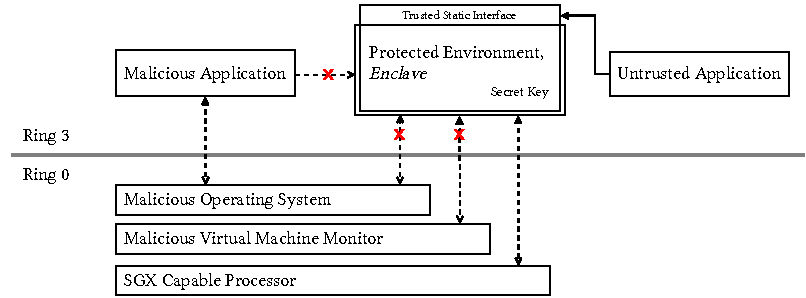
\includegraphics[width=0.95\linewidth]{figures/SGX-architecture.pdf}
    \caption{Abstract overview of SGX's protection in an adversarial environment.}
    \label{fig:sgx-basic}
\end{figure}

\paragraph{} At its heart SGX is designed to be \textit{trustworthy}; this is achieved in a number of ways, including robust enclaving provisioning, sealing and attestation. Intel enumerates SGX's protections~\cite{10.1145/2487726.2488368,sgx-eval-sdk} as follows;

\begin{itemize}
    \item Memory is secured against observation and modification from outside the enclave, achieved using an in-die \textit{Memory Encryption Engine} (\textit{MEE}),~\cite{sgx-mee} with a secret that rotates on every boot. This protection notably works against host hypervisors, other enclaves, and anything running in supervisor mode.
    \item Enclaves can \textit{attest to}, or prove, their identity to a challenger with the help of a permanent hardware security key for asymmetric encryption.
    \item Software calls are proxied to prepare and transfer control in and out of an enclave. Arguments are securely marshalled according to a static enclave definition.
    \item SGX does not defend against reverse engineering or side-channel attacks:~\cite{10.1109/SP.2015.45} this is the responsibility of the developer to mitigate.
    \item Debugging support is only provided via a specialised tool and only when an enclave is compiled with debugging enabled.
\end{itemize}

\subsection{Architecture and Implementation}

\begin{figure}[]
    \centering
    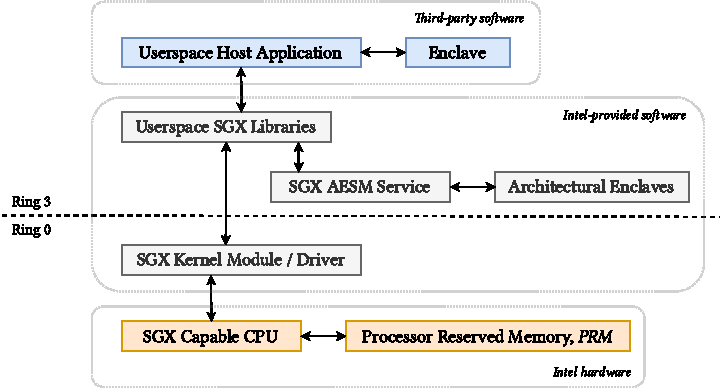
\includegraphics[width=0.9\linewidth]{figures/SGX-AdvArchitecture.pdf}
    \caption{A high-level overview of the SGX hardware and software architecture.}
    \label{fig:sgx-advarch}
\end{figure}

\paragraph{} The SGX platform comprises several interlocking parts (Figure~\ref{fig:sgx-advarch}), building on the core extended x86 instruction set. Information here as reported by~\cite{sgx-sgx-reference,Costan2016IntelSE}.

\subsubsection{Hardware}
\paragraph{} Enclaves' state is stored securely in \textit{Processor Reserved Memory}, \textit{PRM}, a set of pages in system memory presided over by the \textit{MEE}. \textit{PRM} consists of two data structures; the \textit{Enclave Page Cache} (\textit{EPC}) and the \textit{Enclave Page Cache Map} (\textit{EPCM}).

\paragraph{} An enclave is defined by its \textit{SGX Enclave Control Structure}, \textit{SECS} --- this is generated when an enclave is created and stored in a dedicated entry in the \textit{EPC}. A \textit{SECS} holds important metadata such as; the enclave's (system-)global identifier, its measurement hash (\texttt{MRENCLAVE}, §~\ref{sec:attestation}) and the amount of memory it is using.

\paragraph{} The \textit{EPCM} provides an index into the \textit{EPC}: it stores access control information, ownership and validity indicators, and a marker for a page's designated use --- this is not accessible from software. 

\paragraph{} Attempts to resolve \textit{PRM} pages are only successful if the CPU is in enclave mode and the \textit{EPCM} corroborates the enclave's ownership of the region; invalid requests are presented with an unused page from generic system memory. Direct Memory Access to \textit{PRM} is always rejected.

\paragraph{} The \textit{EPC} is managed by the system's hypervisor or OS as typical memory, but must do so using SGX-specific instructions. This is to appease the \textit{MEE}, which is responsible for ensuring the integrity and confidentiality of this process, encrypting and decrypting pages as they cross the \textit{PRM} boundary. An SGX driver, \textit{isgx}, is required to allow userspace applications to use the platform and create/manage enclaves.


\subsubsection{Userspace Services}
\paragraph{} Starting an enclave requires a \textit{launch token} to be retrieved from Intel's \textit{Launch Enclave}; this checks the signature and identity of the enclave to ensure it is valid. Access to the \textit{Launch Enclave} and other architectural enclaves is provided by the AESM service; the userspace SGX libraries facilitate the communication mechanism. Other architectural enclaves include;

\begin{itemize}
    \item The \textit{Provisioning Enclave} --- this verifies the authenticity of the platform and retrieves an enclave's \textit{attestation key} from the \textit{Intel Provisioning Service's} servers.
    \item The \textit{Quoting Enclave} --- this provides trust in the identity of the SGX environment and enclave being attested, by converting the locally generated \textit{attestation key} to a remotely-verifiable \textit{quote}.
\end{itemize}

\subsubsection{Third-party enclaves}
\paragraph{} Enclaves can only be entered via userspace, as detailed in §~\ref{sec:sgx-lifecycle}, and are always accompanied by a host application which acts as its untrusted counterpart. The host application calls the SGX SDK to build an enclave on its behalf using an enclave image, packaged as a standard shared library (\texttt{enclave.so}) and returns its \textit{global identifier}. Control is passed from the host application to the enclave by invoking an enclave function via an \textit{ECALL}. Execution flow can temporarily leave the enclave if it calls one of the host application's functions via an \textit{OCALL}. Execution naturally leaves enclave-mode when an \textit{ECALL} terminates. Both \textit{ECALLs} and \textit{OCALLs} are defined statically in the enclave's interface definition (\texttt{enclave.edl}), and the necessary glue code is generated by the SGX SDK's build toolchain at compile time; this ensures calls crossing the enclave boundary are marshalled safely and correctly.


\subsection{Enclave Lifecycle}
\label{sec:sgx-lifecycle}

\paragraph{} SGX instructions can be separated into two distinct groups; privileged and unprivileged. These, alongside a description of the function they perform, are enumerated in Table~\ref{table:sgx-instructions}.\footnote{A handful of instructions not relevant to the explanation given here are omitted.} The following description of the process of creating an enclave is illustrated in Figure~\ref{fig:sgx-enclavecreate}.

\paragraph{Preparing an enclave} Execution begins with the host application; is needs to initiate the creation process, but must do so via a component with \textit{Ring 0} privilege. This facility is provided by \textit{isgx}, the SGX driver. The application first requests \textit{isgx} to allocate the requisite number of pages to run the enclave $\langle 1 \rangle$;\footnote{These numbers correspond to events in Figure~\ref{fig:sgx-enclavecreate}.} this is tracked and served from the driver's internal state $\langle 2 \rangle$.

\paragraph{} The application continues by executing \texttt{ECREATE} with the metadata of the enclave to be loaded $\langle 3 \rangle$; the \textit{MEE} checks that the pages being claimed are in fact vacant and populates the \textit{SECS} page with the necessary information $\langle 4 \rangle$. Once this is complete the application prepares the remaining \textit{EPC} pages using \texttt{EADD} $\langle 5 \rangle$ and loads the enclave's code and data $\langle 6 \rangle$.

\paragraph{} At this point the enclave needs to be measured --- the application calls \texttt{EEXTEND} $\langle 7 \rangle$, triggering the \textit{MEE} to update the measurement hash in the \textit{SECS} to aligns with the current state of the enclave's memory $\langle 8 \rangle$. Once the \textit{EPC} memory is prepared the application requests for it to be finalised using \texttt{EINIT} $\langle 9 \rangle$: this operation requires the application to retrieve the \texttt{EINITTOKEN} from the \textit{Launch Enclave}, locking the execution of the measured enclave to the CPU the token is generated on. Notably, pages cannot be added after \texttt{EINIT},\footnote{This is only strictly true in SGXv1, as explained in §~\ref{sec:sgx-versions}.} and an enclave cannot be attested to or entered before it. Finally, the initialised flag is set in the \textit{SECS} and the enclave's hash updated for the final time $\langle 10 \rangle$.


\begin{figure}[]
    \centering
    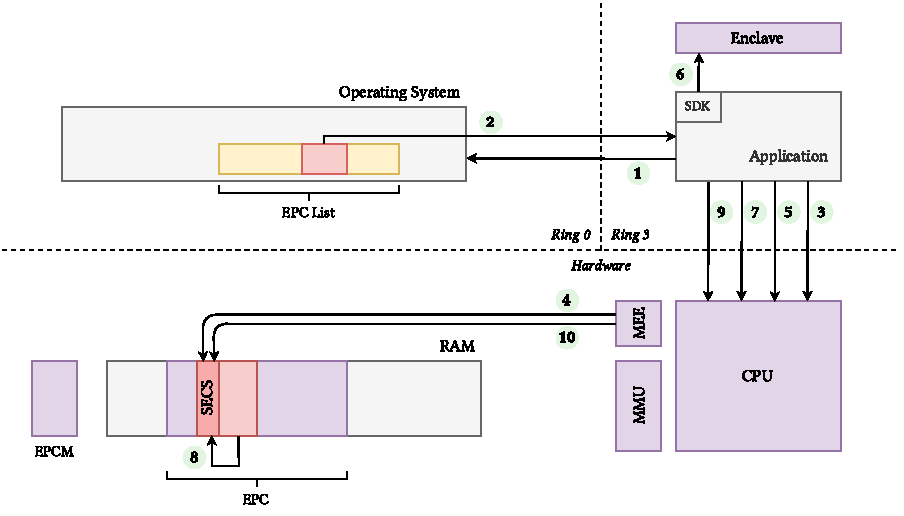
\includegraphics[width=\linewidth]{figures/SGX-EnclaveCreate.pdf}
    \captionsetup{justification=centering}
    \caption[The process of creating and initialising an enclave.]{The process of creating and initialising an enclave; details given in §~\ref{sec:sgx-lifecycle}. Purple components belong to the SGX platform.}
    \label{fig:sgx-enclavecreate}
\end{figure}

\paragraph{Stepping into the enclave} Once an enclave is created it can be invoked using the \texttt{EENTER} instruction; this can only jump to code explicitly defined in the enclave's interface definition and switches the CPU core to enclave mode. SGX uses a flag in the CPU core's \textit{Thread Control Block} to prevent any other logical core following the current one into the enclave.

\paragraph{} Interrupts and exceptions can be served to the enclave, just as with any other application. However, control is not immediately passed over to the defined handler. Instead, the enclave's current state is saved and cleared to ensure no data is leaked. The \textit{Asynchronous Enclave Exit} routine is then invoked and enclave mode disabled. Execution post-interruption is restarted with the \texttt{ERESUME} instruction. Once an enclave has finished executing the registers are erased and \texttt{EEXIT} called. Enclaves are terminated using the \texttt{EREMOVE} command; all claimed \textit{EPC} pages are marked as invalid and the \textit{SECS} page deleted.

\paragraph{} \label{sec:sgx-no-kernel-mode} A significant design decision made in the SGX architecture is that enclaves cannot be entered by a process operating in \textit{Ring 0};~\cite{sgx-prog-reference} the required instructions simply aren't available. This forces all host applications to run in userspace, making interoperation with the kernel challenging, as will be discussed in §~\ref{sec:design}.

\begin{table}
    \centering
    \newcommand\tableTop{\rule{0pt}{3ex}}
    \newcommand\tableMid{\rule{0pt}{3ex}}
    \newcommand\tableBottom{\rule[-2ex]{0pt}{0pt}}
    \begin{tabular}{|c|r|p{8.5cm}|} 
        \hline
        Execution Mode & Instruction & Function \\ [0.1ex] 
        \hline\hline
        \multirow{11}{*}{Ring 0} 
            & \tableTop{\texttt{ECREATE}} & \tableTop{Generate and copy the \textit{SECS} structure to a new page in the \textit{EPC}, initialising a new enclave.} \\ 
            & \texttt{EADD} & \tableMid{Add a new \textit{EPC} page for the current enclave; this is used to load initial code and data.} \\ 
            & \texttt{EEXTEND} & \tableMid{Updates the enclave's measurement during attestation; modifies the \textit{SECS}.} \\ 
            & \texttt{EINIT} & \tableMid{The terminal instruction in an enclave's initialisation, finalising its attributes and measurement.} \\ 
            & \texttt{EREMOVE} & \tableMid{Permanently remove a page from the \textit{EPC}; usually invoked during enclave destruction.} \tableBottom \\ 
        \hline\hline
        \multirow{11}{*}{Ring 3} 
        & \tableTop{\texttt{EENTER}} & \tableTop{Transfer control from the host application to a pre-determined location in an enclave.} \\ 
        & \texttt{ERESUME} & \tableMid{Re-enter the enclave after an interrupt/exception and resume execution.} \\ 
        & \texttt{EEXIT} & \tableMid{Restore the original operating mode at the location \texttt{EENTER} was triggered and flush the TLB.} \\ 
        & \texttt{EGETKEY} & \tableMid{Access platform cryptography keys required for attestation and sealing.} \\ 
        & \texttt{EREPORT} & \tableMid{Generate a \textit{report} for an enclave's \textit{attestation key} for an attestation process.} \tableBottom \\ 
        \hline
    \end{tabular}
    \vspace{5mm}
    \caption[Overview of notable SGX x86 instructions in an enclave's lifecycle.]{Overview of notable SGX x86 instructions in an enclave's lifecycle.~\cite{sgx-prog-reference}}
    \label{table:sgx-instructions}
\end{table}


\subsection{Attestation}
\label{sec:attestation}

\paragraph{} An essential feature of the \textit{trusted computing} model SGX creates is attestation, the process of verifying both the authenticity and integrity of components cryptographically. SGX achieves by creating two hashed values, or \textit{signing identifiers}, per enclave; \texttt{MRENCLAVE} and \texttt{MRSIGNER}.~\cite{Anati2013InnovativeTF,sgx-prov-service}

\paragraph{} \texttt{MRENCLAVE} acts an a unique identifier for the contents of an enclave. It is generated by hashing the instructions and data passed when creating the enclave with \texttt{ECREATE}, \texttt{EADD}, and \texttt{EEXTEND}; the value is finalised and stored in the \textit{SECS} on \texttt{EINIT}. This value depends on the exact content and ordering of the enclave's \textit{EPC} pages. As long as the enclave's source remains the same, so will its \texttt{MRENCLAVE}.

\paragraph{} \texttt{MRSIGNER}, also known as the enclave's \textit{Sealing Identity}, is generated during the enclave build process --- all production enclaves need to be signed using an RSA key provided by the compiling user (the \textit{Sealing Authority}). The public key from this pair is stored in \textit{SIGSTRUCT}, the \textit{Enclave Signature Structure}. During an enclave's launch its signed compile-time \texttt{MRENCLAVE} value (held in \textit{SIGSTRUCT}) is decrypted and crossreferenced with a freshly-computed runtime \texttt{MRENCLAVE} value to detect tampering. \texttt{MRSIGNER} is the same for all enclaves signed by the same \textit{Sealing Authority}.

\paragraph{Local Attestation} Two enclaves resident on the same system are able to attest their identities to each other using their \texttt{MRENCLAVE} and \texttt{MRSIGNER} values; this usually precedes the establishment of a shared secret (using a variant of \textit{Diffie-Hellman} backed by the platform's master SGX key)\footnote{Note for Harri: must check these details.} for confidential communication between them.

\paragraph{Remote Attestation} In addition to attestation between entities on the same platform, the Intel specification also provides a workflow for an enclave to attest its identity to a remote party. The system's \textit{Quoting Enclave} verifies an enclave's local \textit{quote} and creates a digital signature of it using the CPU's permanent hardware SGX private key. Through the use of an \textit{Intel Enhanced Privacy Identifier} (\textit{EPID})~\cite{epid} this process can be carried out anonymously; it relies on information encoded in the CPU during the manufacturing process. The \textit{Provisioning Enclave} assists in this process, especially as production enclaves are required to attest with Intel's provisioning service~\cite{sgx-prov-service} before executing. Remote attestation is not explicitly required in this project's architecture hence will not be covered in any further detail.

\subsection{Sealing}
\label{sec:sealing}
\paragraph{} \textit{Sealing} refers to the encryption of data using a key related to the generating enclave; this key is unique to that enclave on a particular platform. SGX offers two policies for deriving the encryption key based on the platform's \textit{Root Sealing Key} --- relative to the current enclave (\texttt{MRENCLAVE}) or the current enclave's \textit{Sealing Authority} (\texttt{MRSIGNER}). These serve many use cases, including, for example, allowing state to persist through enclave upgrades.

\subsection{SGX Versions}
\label{sec:sgx-versions}
\paragraph{} At the time of writing there are two versions of SGX available, \textit{v1} and \textit{v2} --- the details given here relate to \textit{v1} as this project will be compatible with both. \textit{v2} offers a number of improvements on which this project does not rely, including: (a) dynamic memory management, (b) eased production enclave restrictions (`Flexible Launch Control'), (c) increased PRM size support, and (d) support for virtualisation.


% -------------

\section{Aspects of the \textit{Linux} Kernel}

\paragraph{} Linux needs little introduction. First created in 1991 as an open-source alternative to UNIX, it now powers over 90\% of \textit{the cloud} and 85\% of smartphones. With almost 25,000 contributors to the kernel, it is immensely complex, with numerous interlocking parts. This section shall provide a brief overview of a small subset of them to support the information given in §~\ref{sec:design}.

\subsection{Virtual File System}

\paragraph{} Linux represents almost every component as a file, for example including sockets, terminals, and driver interfaces. The role of providing this abstraction falls to the VFS, the core function of which is as a transparent layer, routing requests to the correct underlying implementation. This virtual interface relies on the following mechanisms.

\paragraph{Superblocks} The \textit{superblock} attached to an entity represents the characteristics and properties of the filesystem in which it sits. The metadata it holds includes: the block size, statistics on available blocks, the size and location of the filesystem inode tables, the disk block map, and block grouping data. An important marker held in the superblock is it's \textit{magic value}; this predefined code\footnote{Defined in \texttt{include/uapi/linux/magic.h}.} indicates the underlying implementation the filesystem belongs to. Examples include \textit{EXT4} (\texttt{EXT4\_SUPER\_MAGIC}), \textit{pseudo terminal devices} (Linux shells, \texttt{DEVPTS\_SUPER\_MAGIC}), or sockets via \textit{SockFS} (\texttt{SOCKFS\_MAGIC}).

\paragraph{Inodes} The \textit{inode} data structure represents information about a single file existing on a file system. All objects, not only files are \textit{backed} by inodes. No pathname is assigned at this level; this is provided at a higher level of abstraction. An inode does however indicate ownership information, access restrictions and content type, and is identified by its \textit{inode number}.

\paragraph{Dentries} Each item in the \textit{direct entry cache} (\textit{dcache}), shortened to \textit{dentry}, represents a connection between an inode and the path it resides at in the VFS. This glue layer is responsible for building the tangible folder structure, and as the name suggests, metadata caching. A \textit{file} consists of a \textit{dentry}-\textit{inode} pair.

\paragraph{File descriptors} Whenever a process opens a file, it is presented with a \textit{file descriptor} by the kernel (via \texttt{open()} or similar). This structure is unique to a process, providing the gateway between the process and the underlying file it describes. All active descriptors can be viewed at \texttt{/proc/<pid>/fd/}; for standard processes \textit{0} globally refers to \textit{stdin}, \textit{1} to \textit{stdout}, and \textit{2} to \textit{stderr}. Reads and writes to a file (or socket, pipe, etc.) are performed on the relevant file descriptor, not the object directly.

\subsubsection{Extended Attributes} 

\paragraph{} Files can have additional, external, key-value pairs attached to them. These attributes, shortened to \textit{xattrs}, are permanent and saved to disk alongside the file's content. Values are optional and may be left empty if the attribute is just a flag, but if a value is specified it must be in the form of a null-terminated string. \textit{xattrs} are namespaced to define different classes of functionality; the \texttt{user} namespace is open to all (e.g. \texttt{user.example\_attribute}), but \texttt{trusted}, \texttt{system}, and \texttt{security} are reserved for specific uses by the kernel --- the \texttt{security} namespace belongs exclusively to LSMs (§~\ref{sec:lsm}).




\subsection{Linux Security Modules}
\label{sec:lsm}

\paragraph{} Linux supports the inclusion of third-party security models in the kernel itself using a unified framework, LSM. This provides developers with \textit{hooks} into kernel functionality at every point a userspace \textit{syscall} is about to access fundamental kernel primitives, such as inodes or task control structures. Each of these hooks can influence to behaviour of the kernel by allowing or denying the operation.

\paragraph{} LSM attaches a \texttt{void*} security field to every instance of kernel primitives, such as \texttt{struct inode}, to allow security implementations to attach additional state to each, tracking them in whatever way is most appropriate. Decisions taken within an LSM affect all aspects of a Linux system; \textit{superuser} privilege cannot override it and every component in the system can be restricted.


\subsubsection{Integrity Measurement Architecture}

\paragraph{} Linux's IMA subsystem is responsible for calculating the hashes of files and programs as they are loaded (\textit{measurement}), verifying them against an allowed list if required (\textit{appraisal}). Its driving purpose is to detect if files have been maliciously altered either remotely or locally; the file's hash is stored as an \textit{xattr} (\texttt{security.ima}). IMA supports many use cases, the majority of which are complementary to the LSM framework, but we shall focus on one here --- EVM.

\paragraph{} The Linux \textit{Extended Verification Module}, \textit{EVM}, hardens IMA by protecting \textit{xattrs} in the \texttt{security} namespace --- this covers both the IMA hash and any labels created by security modules. Two tamper-detection methods are provided:

\begin{enumerate}
    \item The \textit{HMAC-SHA1} hash of the \texttt{security} namespace is stored as \texttt{security.evm} for reference, and
    \item A digital signature of this value is stored alongside using a key that is sealed either using a \textit{TPM}\footnote{Trusted Platform Module.~\cite{tpm}} or passphrase.
\end{enumerate}

\textcolor{red}{Need to reference in the evaluation.}

\chapter{Related Work} 
\paragraph{} This is my related works

\chapter{Design and Implementation}


\paragraph{} In this chapter we shall introduce and detail a prototype implementation of a modular, SGX-protected \textit{reference monitor} --- \textsc{Citadel}. We start by considering this project's motivation and discussing the challenges faced. Then, we explain the three-part architecture, relating design decisions to its DIFC model. We discuss the architecture's performance and effectiveness in §~\ref{sec:eval}.

\section{Motivation}
\paragraph{} Since its introduction in Anderson's 1972 report,~\cite{reference-monitor} the reference monitor concept has proved a reliable workhorse for many security models. It does not refer to any exact policy, nor limit itself to any particular implementation --- its abstractness is one of its greatest strengths, reserving any judgement about what policy is \textit{appropriate} in a particular setting.~\cite{irvine-rm}

\paragraph{Fundamental Properties of a Reference Monitor}

\begin{itemize}
    \item \textit{Always invoked.} To guarantee that adversaries are unable to bypass the system's security policies, every access to the system must be mediated
    \item \textit{Evaluable.} It ``must be small enough to be subject to analysis and tests, the completeness of which can be assured'';~\cite{reference-monitor} to be trustworthy, it must be \textit{auditable}, with, ideally, a restricted TCB.
    \item \textit{Tamper proof.} To ensure that an attacker cannot disable the authorisation mechanisms mandated by the security policy, the integrity of a reference monitor cannot be in question.
\end{itemize}

\paragraph{} No computer system is ever completely secure, and Linux is no exception. Having grown by 1.7 million lines of code (LoC) in the past year alone, to 27.8 million LoC in total,\footnote{\url{https://www.theregister.com/2020/01/06/linux\_2020\_kernel\_systemd\_code/}} bugs are inevitable --- almost 2000 have been reported in the past year,\footnote{\url{https://bugzilla.kernel.org/}} and 662 \textit{severe} bugs are still outstanding.\footnote{\url{https://www.cvedetails.com/product/47/Linux-Linux-Kernel.html}} Therefore we must question whether Linux alone can provide a reference monitor implementation the guarantees it requires,~\cite{Lipp2018MeltdownRK, 10.5555/2831143.2831164} thus motivating the use of SGX.

\paragraph{} Applying SGX to this problem brings two attractive benefits;
\begin{itemize}
    \item The system's IFC policy can be evaluated both during offline analysis and online using \textit{attestation}, building other enclaves' confidence in the underlying system.
    \item SGX's hardware protections are very capable of defending a reference monitor's state, even if adversaries have ring-0 privileges or in the presence of a kernel bug.
\end{itemize}

\section{Challenges}
\label{sec:challenges}

\begin{figure}[]
    \centering
    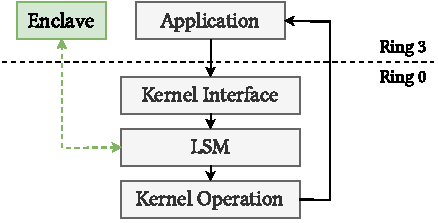
\includegraphics[width=0.48\linewidth]{figures/SGX-EnclaveIntegration.pdf}
    \caption{Abstract \textit{syscall} control flow route. Grey components show the natural Linux design. Green additions highlight the externalised enclave LSM component.}
    \vspace{5mm}
    \label{fig:sgx-abstract-integration}
\end{figure}

\paragraph{} The natural location for a reference monitor is embedded directly into the kernel, in the path of \textit{syscalls'} control flows. \textit{CamFlow} does this using the LSM framework, silently tagging processes and other entities as they are encountered by the kernel, and additionally providing an external LSM-interface for any active changes. However, an SGX enclave is incompatible with this workflow (§~\ref{sec:sgx-no-kernel-mode}) as it cannot execute alongside kernel code. Thus a significant, unavoidable design feature is that the reference monitor must be distributed across rings 0 and 3 --- an enclave \textit{policy} component, and an LSM for \textit{enforcement}.

\paragraph{} The disruption this change causes could severely impact performance; Figure~\ref{fig:sgx-abstract-integration} highlights the significant change to overall control flow. Most notably, externalising part of the LSM to an enclave forces, in the worst case, an additional pair of context switches for each \textit{syscall}.

\paragraph{} Given a ring-3 component is unavoidable, we seek to minimise the overhead caused by its integration, while maintaining \textit{safety} (every operation must be mediated). This problem is reminiscent of the ones that inspired the development of \textit{exokernels}~\cite{10.1145/224056.224076} --- both the drawbacks and opportunities of those approaches apply here.~\cite{10.1145/269005.266644} 
% TODO
% \textcolor{red}{More detail about why.}

\paragraph{} Two architectures, as illustrated in Figure~\ref{fig:sgx-integration}, were initially considered. 

\begin{enumerate}
    \item An \textit{isolated} extension of the LSM. Only the security implementation communicates with the \textit{policy} enclave, acting as a na\"{i}ve reimplementation of a fully self-contained LSM, and using an additional kernel module as an I/O relay.
    \item An \textit{integrated} userspace service, through which permission is \textit{requested} ahead of time and decisions stored in the LSM until needed. Backflow of information is facilitated asynchronously, but no additional kernel relay is required.
\end{enumerate}



\begin{figure}[]
    \centering
    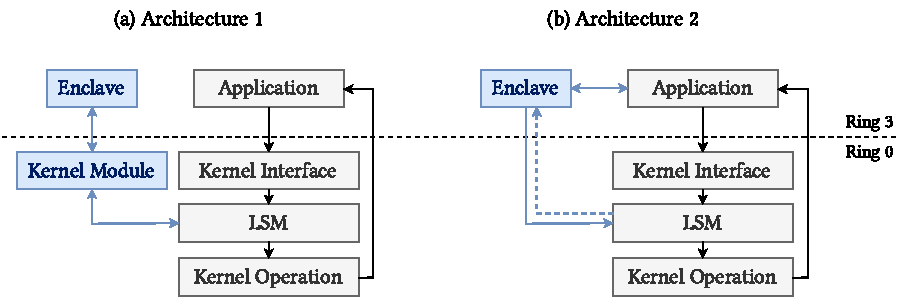
\includegraphics[width=0.98\linewidth]{figures/SGX-EnclaveIntegration-Design}
    \caption{Two possible enclave integration designs.}
    \vspace{2mm}
    \label{fig:sgx-integration}
    \vspace{5mm}
\end{figure}

\paragraph{}\textit{Architecture 1} can be implemented without changing the IFC model presented in §~\ref{sec:ifc-modelling}, reducing concerns regarding correctness and safety. However it adds significant overhead to the critical sections~\cite{Dubois1988SynchronizationCA} of core LSM functions, in most cases while the kernel holds locks for various objects being accessed.

\paragraph{} \textit{Architecture 2} is more flexible, requiring all negotiation be conducted ahead of time, and importantly, without leaving userspace: any overhead only impacts the application, leaving the kernel's critical sections to execute with minimal interference. A notable downside, however, is that the system's security model will need an extension because \textit{policy decisions and enforcement are no longer one and the same}.

\paragraph{} Preliminary experiments showed that performance of the two architectures was similar in light workloads, but that \textit{Architecture 1} degrades significantly due to resource contention. Additionally, as will be explained in §~\ref{sec:citadel-tcb}, the dependence on a kernel module conflicts with the desired constrained TCB of the system. For these reasons \textit{Architecture 2} forms the basis of the prototype.

\paragraph{} An additional challenge is one of incomplete information --- an enclave is not privy to internal kernel datastructures such as \texttt{task\_struct}, which will store the taint and capabilities of processes. A potential solution would be a request---response model via a custom kernel interface for any queries, though the performance impact would be severe, requiring additional context switches. Instead, the approach adopted creates an abstract interface that purposefully removes the minutiae of the underlying system. Any solution must be trustworthy and safe, and malicious entities must not be able to exploit any \textit{eventually consistent} components.~\cite{10.1145/1435417.1435432}

\paragraph{} As a final comment, it must be noted that SGX is not flawless; §~\ref{sec:sgx-vulnerabilities} discusses the impact of this on the project.


% ---------------

\section{The \textsc{Citadel} IFC Model}

\paragraph{} Before work on the final \textsc{Citadel} implementation began, we constructed a formalisation describing the distributed nature of its design. A model helps reason about the safety and correctness of the final system, and provides the notation to properly discuss its features. Our model directly extends the one presented in §~\ref{sec:ifc-modelling}.

\subsection{Reservations}

\paragraph{} Previously we defined the concept of a \textit{safe flow}, $A \rightarrow B$, which underpins our IFC restrictions. In previous works permission is granted while \textit{implicitly} considering \textit{how} the flow is to take place (\ref{eqn:res-1}). An isolated \textit{enforcement} component does not understand the concept of \textit{flows}, forcing policy decisions to be defined \textit{explicitly}; \textsc{Citadel} uses \textit{reservations} for this purpose (\ref{eqn:res-2}). This distinction is simple but very important when introducing \textit{laziness} and other optimisations between the two halves of the reference monitor.

\begin{equation}\label{eqn:res-1}
    \textit{operation} \rightarrow \boxed{\textit{reference monitor}} \xrightarrow{\;\;\textit{decision}\;\;} \{0,1\}
\end{equation}
\vspace{-3mm}
\begin{equation}\label{eqn:res-2}
    \textit{operation} \rightarrow \boxed{\textit{policy}\; \xrightarrow{\;\;\textit{reservation}\;\;} \;\textit{enforcement}} \xrightarrow{\;\;\textit{decision}\;\;} \{0,1\}
    \vspace{3mm}
\end{equation}


\paragraph{} Let $\Omega$ be the set of all operations mediated by the reference monitor, for example, \texttt{file\_read} or \texttt{socket\_open}, and $\mathcal{R}$, the set of all \textit{reservations}, as follows.\footnote{Recalling that $\mathcal{T}$ is the set of all tags.}

\newcommand{\powerset}{\raisebox{.15\baselineskip}{\Large\ensuremath{\wp}}}
\vspace{-5mm}
\begin{equation*}
    \mathcal{R} = \mathcal{T} \times \powerset(\Omega)
    \vspace{2mm}
\end{equation*}

\paragraph{} Further, we define a shorthand, $t^{\alpha}$;
\vspace{-3mm}
\begin{equation*}
    r \in \mathcal{R} \;.\; (r = (t, \alpha) = t^{\alpha} \implies t \in \mathcal{T} \; \wedge \; \alpha \subseteq \Omega)
\end{equation*}

\paragraph{} For a process $A$, $A_{r} \subseteq \mathcal{R}$ defines the set of all reservations it holds. Once a decision has been made, it is important for a reference monitor to be able to change it, revoking access if required. Thus we specify \textit{validity} with an indicator function, $\mathcal{V}: \mathcal{R} \mapsto \{0,1\}$. A reservation can only be used if valid; invalid reservations are discarded.

\subsection{Permissible Operations}
\label{sec:permissible-operations}

\paragraph{Satisfiability} To determine if an operation is permissible, the \textit{constraint reservation} representing it is compared against reservations held by the process. For example, $t^{\{\texttt{file\_read}\}}$ is the constraint for reading a file tagged $t$.

\paragraph{} A constraint $\tau^{x}$ is said to be satisfied by a reservation $\tau^{y}$ ($\tau^{x} \sprecsim \tau^{y}$) if the tags match, the reservation is valid, and $y$ permits \textit{at least} the required form of access (\ref{eqn:satis-1}). 

% Equations (\ref{eqn:satis-2}) and (\ref{eqn:satis-3}) define set comparison counterparts --- constraint $\tau^{x}$ is satisfied by a set of reservations $y$ ($\tau^{x} \sqin y$), and a set of constraints $\mu$ is satisfied by a set of reservations $\nu$ ($\mu \sqsubseteq \nu$).

\vspace{-5mm}
\begin{align}
    \sigma^{\alpha}, \tau^{\beta} \in \mathcal{R} &\;.\; (\; \sigma^{\alpha} \sprecsim \tau^{\beta} \iff \sigma = \tau \;\wedge\; \alpha \subseteq \beta \;\wedge\; \mathcal{V}(\tau^{\beta}) \;) \label{eqn:satis-1}
\end{align}

% \\
% \sigma^{\alpha} \in \mathcal{R}, \; x \subseteq \mathcal{R} &\;.\;  (\; \sigma^{\alpha} \sqin x \iff \exists \, \tau^{\beta} \in x \;.\; \sigma^{\alpha} \sprecsim \tau^{\beta} \;) \label{eqn:satis-2}\\
% \mu, \nu \subseteq \mathcal{R} &\;.\;  (\; \mu \sqsubseteq \nu \iff \forall \, \alpha \in \mu \;.\; \alpha \sqin \nu \;) \label{eqn:satis-3}

\paragraph{} From here we define a \textit{permissible operation}, $A \xrightharpoonup{\;\omega\;} t$; process $A$ may perform operations $\omega$ on an entity tagged $t$. An operation is only permissible if the process holds a reservation explicitly granting permission (\ref{eqn:permissible-op}).
\begin{equation}
    \label{eqn:permissible-op}
    A \xrightharpoonup{\;\omega\;} t \iff (\exists \; t^{\alpha} \in A_r \implies t^{\omega} \sprecsim t^{\alpha})
\end{equation}

\paragraph{} To bridge the gap between permissible flows and operations, a final definition is required; a \textit{specific permissible flow}, $A \,\xmapsto{\;\omega,\tau\;}\, B$, meaning that $A$ may send information to $B$ using operations $\omega$, via entities tagged with $\tau$. Thus:

\vspace{-7mm}
\begin{align}
    (\exists\, \omega,\tau \;.\; A \,\xmapsto{\;\omega,\tau\;}\, B) \implies & A \rightarrow B \\
    A \,\xmapsto{\;\omega,\tau\;}\, B \implies & (\exists \,\omega' \;.\; A \xrightharpoonup{\;\omega'\;} \tau \;\land\; \omega \subseteq \omega') \label{eqn:flow-abs-conc-map}
\end{align}

\paragraph{} Together, these define the relationship between an abstract policy space ($A \rightarrow B$, §~\ref{sec:policy-enclave}) and concrete implementation ($A \xrightharpoonup{\;\omega\;} \tau$, §~\ref{sec:enforcement-domain}). A policy decision may grant a greater set of permissions than asked for (\ref{eqn:flow-abs-conc-map}) --- e.g. allowing both read and write when only write was explicitly requested.~\cite{flume,Zeldovich2008}

\paragraph{} Some small updates are required to make the existing rules consistent with the new: reservations are not transferred when creating a new entity (\ref{eqn:new-creation}), and reservations are not affected by capabilities as they represent a centralised component of the DIFC system. 

\vspace{-5mm}
\begin{equation}
    A \Rightarrow B \implies A_s = B_s \; \wedge \; A_i = B_i \; \wedge \; B_r = \varnothing \label{eqn:new-creation}
\end{equation}


\subsection{Transient Entities}
\label{sec:transient-entities}

\paragraph{} Alongside active and passive entities, we introduce a third type; \textit{transient} entities. These are passive entities that are privately held by an owning active entity; they are used to model Linux functions such as \texttt{pipe()} and unclaimed tainted files.

\paragraph{} To facilitate this, all processes are assigned a unique tag $p \in \mathcal{T}$, and any files it creates are initially also be tagged with $p$. Using $\mathcal{P}$ as the set of all process identifiers, we define $\mathcal{I}$ as the function returning a process's transient identifier;

\vspace{-5mm}
\begin{equation}
    \mathcal{I}: \mathcal{P} \mapsto \mathcal{T}
\end{equation}

\paragraph{} The expression for a \textit{permissible operation} now becomes;

\vspace{-5mm}
\begin{equation}
    A \xrightharpoonup{\;\omega\;} t \iff \mathcal{I}(A) = t \;\lor\; (\exists \; t^{\alpha} \in A_r \implies t^{\omega} \sprecsim t^{\alpha})
\end{equation}

% ---------------
\clearpage
\section{Implementation}

\begin{figure}[]
    \centering
    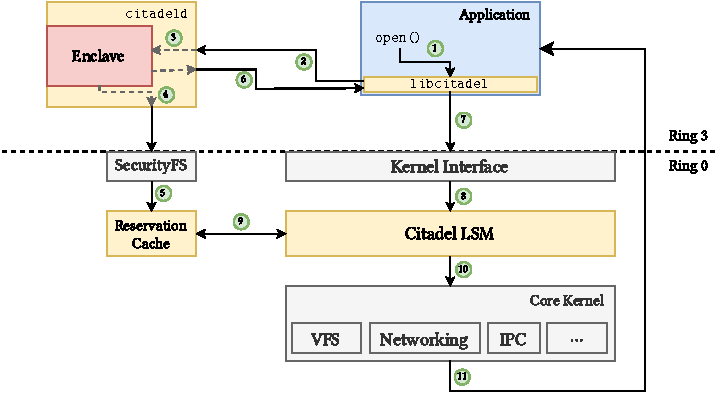
\includegraphics[width=\linewidth]{figures/OverallArchitecture.pdf}
    \caption{High level overview of the \textsc{Citadel} architecture.}
    \vspace{-5mm}
    \label{fig:citadel-overview}
    \vspace{5mm}
\end{figure}

\paragraph{} \textsc{Citadel} consists of three components; an LSM, \texttt{citadeld}, and \texttt{libcitadel}. Each plays an essential, symbiotic role in the operation of the reference monitor. The prototype is in excess of 9,000 lines of C and C++, and extends the Linux kernel build system (§~\ref{sec:build-system}). This section shall present \textsc{Citadel}'s architecture, guided by Figure~\ref{fig:citadel-overview}.

\paragraph{Analogy} The system is well illustrated by the \textit{will-call} system used by theatres --- customers (\textit{processes}) reserve tickets (\textit{permission}) to attend a show (\textit{perform an operation}) ahead of time via phone or the internet (\texttt{citadeld}), but only receive their tickets (\textit{reservations}) at the venue (\textit{LSM}) on the day (\textit{at the point of execution}).

\paragraph{} \textsc{Citadel}'s LSM comprises its \textit{enforcement domain} (§~\ref{sec:enforcement-domain}), and \texttt{citadeld} its \textit{policy domain} (§~\ref{sec:policy-enclave}). Enforcement is \textit{policy-agnostic}, implementing an abstract, tagged taint tracking system that exposes decision points to policy influence via reservations. Policy components need not be aware of the enforcement strategy to successfully express their protection schemes. Communication between the two domains is discussed separately in §~\ref{sec:interdomain-comms}.



\subsection{Enforcement}
\label{sec:enforcement-domain}

\begin{figure}[]
    \centering
    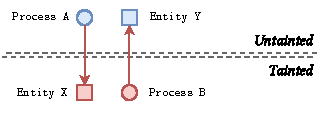
\includegraphics[width=0.55\linewidth]{figures/CitadelTaint.pdf}
    \caption[Accesses across the taint boundary]{Accesses across the taint boundary taint the untainted party.}
    \label{fig:taint-boundary}
\end{figure}

\paragraph{} The \textsc{Citadel} LSM tracks all entities within the Linux system by allocating and attaching a small data structure ($<48$ bytes) to each; it computes and tracks a conservative notion of \textit{taint} for each to ensure \textit{safety}. Tainting in \textsc{Citadel} is dynamic, meaning that entities are only policed if needed. This process is \textit{additive}, only tainting an object if it is involved in a successful operation crossing the taint boundary (Figure~\ref{fig:taint-boundary}). In additional to automatic propagation, taint for the majority of entities is amendable on request from the policy domain.

\paragraph{} A variety of metadata is tracked for each type of entity:

\begin{enumerate}
    \item[---]\textbf{Active}. The only active entities in Linux are processes --- these require a plethora of markers and flags, including; \textit{taint} and its \textit{reservation list}.
    \item[---] \textbf{Passive}. There are many forms of passive entity, the most prevalent being files and other inode-backed structures. These carry \textit{taint}, an \textit{identifier} (tag), and an \textit{anonymous flag}. Inode tracking is detailed first, with other types of passive entities, such as shared memory, discussed in §~\ref{sec:shm}.
\end{enumerate}

\subsubsection{Identifiers}
\paragraph{} Entities may be tagged with a single identifier; a randomly assigned 128-bit number which corresponds to a tag in the IFC model. If a security policy wishes to maintain pseudonyms for secrecy and integrity, for example, it may internally, but must convert back to the system tag for enforcement.

\subsubsection{Extended Attributes} 
\paragraph{} An inode-backed entity's taint flag and identifier are copied to \textit{xattrs} attached to it via the VFS. These occupy the \texttt{security.citadel} namespace, and are essential for ensuring that taints and identifiers persist between boots. Certain entities may be \textit{anonymous}, indicated by an anonymous flag, meaning that their identifier is not present as an \textit{xattr}. This may either be because the entity does not support \textit{xattrs} (such as files created using \texttt{pipe()}) or that the identifier is temporary (§~\ref{sec:entity-creation}).


\subsubsection{Permissions} 
\paragraph{} Tainted processes must hold a valid reservation to perform any operation that may allow data to flow to another entity (Appendix X) --- enforcement strictly follows the rules presented in §~\ref{sec:permissible-operations}. Untainted processes bypass all checks, and thus lie outside the IFC model; the security implications of this are discussed in §~\ref{sec:ifc-model-implications}


\subsubsection{Reservation Cache} 
\paragraph{} When the system's policy enclave presents a new reservation to the LSM, it is stored in a structure called the \textit{reservation cache}. Implemented as a red-black tree, this maps a process's identifier to a linked list of its pending reservations. This intermediary storage is necessary as LSMs are event-driven, and thus can only access an entity's state when it is presented for review. Before a permission check is carried out, the LSM ensures that the process's reservation list is up to date by;
\begin{enumerate}
    \item \textit{Installing pending tickets}. All reservations held for the process are moved to its internal reservation list, ready for inspection.
    \item \textit{Disposing of expired entries}. The validity function the LSM uses is time-based. When a reservation is inserted into the reservation cache, it is timestamped with an explicit expiry date --- this lifetime is $15$ seconds by default.  
\end{enumerate}


\subsubsection{Entity Creation}
\label{sec:entity-creation}
\paragraph{} As detailed in §~\ref{sec:transient-entities}, every newly spawned process is privately tagged by the LSM as if it were a passive entity. The purpose of this identifier is not to directly identify the process, but to provide a mechanism for associating any private, passive entities it creates with it. This includes the file descriptors provided by \texttt{pipe()}, and any new files it creates using \texttt{open()}. Every process always has permission to access its transient entities, and external entities can only gain the right to access them if they;
\begin{enumerate}
    \item Are a child processes and request access to their parent, or
    \item The process officially \textit{claims} them via the policy enclave, which gives them an independent tag and removes the entity's status as transient. 
\end{enumerate}


\paragraph{\texttt{fork()}} In Linux, child processes are initially exact clones of their parent, with access to the same state and file descriptors. Thus children of tainted processes are also tainted, but importantly do not assume the same rights as their parents --- open file descriptors will not function without revalidation (§~\ref{sec:libcitadel}), and children must request the right to their parent's transient entities to use pipes or similar.\footnote{Unrelated processes are unable to do this.} It is the policy enclave's responsibility to validate that the security contexts of the parent and child have not diverged. 
% TODO
% \footnote{\textcolor{red}{mention leakage through fd state}}





\subsection{Policy Components}
\label{sec:policy-enclave}

\paragraph{} The policy counterpart to the LSM's enforcement is contained within \texttt{citadeld}, a userspace service that hosts the core SGX enclave. \texttt{citadeld} is modular, hosting an independent policy module sitting on top of an enforcement translation library (Figure~\ref{fig:policy-enclave}).

\subsubsection{Abstract Policy Module}
\paragraph{} The policy module embedded in \texttt{citadeld} is presented with a simple, event-driven interface; this streamlines their implementation, allowing more emphasis to be put on correctness. Their implementation is based around a single method, through which their permission is sought when required; \texttt{asm\_handle\_request(3)}.


\paragraph{} The simplest possible policy is that any operation is deemed permissible. The request parameter, amongst other things, holds the target identifier and set of operations. 

\vspace{3mm}
\begin{minted}[fontsize=\small]{c}
citadel_response_t asm_handle_request (pid_t pid, 
        struct citadel_op_request *request, void *metadata) {
    return CITADEL_OP_APPROVED;
}
\end{minted}

\begin{figure}[]
    \centering
    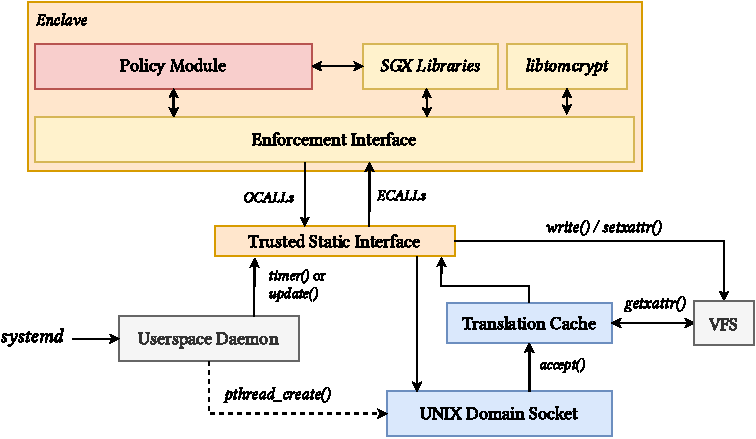
\includegraphics[width=0.9\linewidth]{figures/EnclaveLayout.pdf}
    \caption{Overview of the components inside \texttt{citadeld}.}
    \label{fig:policy-enclave}
\end{figure}

\paragraph{} This can be considered to determine the validity of an operation, $A \xrightharpoonup{\;\omega\;} t$, based on its knowledge of any implicated flows ($A \rightarrow *$).

\paragraph{Operations} Entity operations, $\Omega$, are presented as \texttt{citadel\_operation\_t}, a simple bit mask over the operations \textsc{Citadel} recognises (Appendix X). Similarly, policy decisions are represented using \texttt{citadel\_response\_t}; these may be \textit{approved}, \textit{rejected}, \textit{error}, \textit{invalid}, \textit{granted},\footnote{Approved, and confirming that the process is recognised as the owner of the entity.} and \textit{forged}.\footnote{Discussed in §~\ref{sec:additional-security}.}


\subsubsection{Host Application}

\paragraph{} Various steps need to be taken before requests are presented to the resident policy module (§~\ref{sec:interdomain-comms}). Requests often refer to absolute filepaths, requiring retrieval of their tags, if they exist --- security \textit{xattrs} attached to the VFS file serve these requests. Translation is performed pre-emptively depending on the operation requested, and to minimise any lookup overhead, results are cached in a \textit{translation cache}. This is implemented using \textit{sparsehash},\footnote{\url{https://github.com/sparsehash/sparsehash}} and great care is taken to detect stale entities that may confuse the internal decision process.


\subsubsection{Enforcement Interface}
\paragraph{} The policy module is interchangeable, but the enforcement interface acts as the backbone of the enclave. All requests are routed through it as a sanitsation step, detecting forgery or invalid data, and all information leaving it is formatted and signed\footnote{Encryption is discussed in §~\ref{sec:interdomain-comms}} as appropriate. The process of installing reservations created by the enforcement interface, on behalf of the policy module, is detailed in §~\ref{sec:interdomain-comms}.

\subsubsection{\texttt{libtomcrypt}}
\paragraph{} We ported \textit{libtomcrypt},\footnote{\url{https://github.com/libtom/libtomcrypt}} a leading open-source cryptography library, to function inside an SGX enclave. This was necessary to support many encryption mechanisms the system requires, on top of those provided by SGX. This was achieved by replacing its backing precision arithmetic library with an SGX-aware version of \textit{GMP},\footnote{\url{https://github.com/intel/sgx-gmp}} and forcing it to statically allocate its memory (as SGX v1 lacks support for dynamic memory management). Further changes rewrote the internal random number generator to use the one provided by SGX, and rework its exception strategy to remove \texttt{abort()}, an illegal instruction inside an enclave.

\subsubsection{Shared Memory}
\label{sec:shm}
\paragraph{} \textsc{Citadel} also supports the tagging and restriction of shared memory (SHM). This is managed not via a backing inode, but directly using \textit{System V} identifiers granted to allocated memory segments. Internally, restrictions function in the same way as files, but per-access mediation is not directly possible -- we can only detect when segments are allocated and attached. Thus this workflow requires special consideration, and a new reporting mechanism from the LSM back to the policy enclave. Using a specialised \textit{xattr} interface (\ref{eqn:shm-interface}) to drive a request-response model, the LSM tracks and reports the PIDs of everything that has touched an SHM segment. 

\vspace{-5mm}
\begin{align}
    \texttt{security.citadel.shm.[shm\_id]} \rightarrow \{145, 267, 1120, ...\} \label{eqn:shm-interface}
\end{align}

\subsection{Communication Pathways}
\label{sec:interdomain-comms}
\paragraph{} There are three notable I/O pathways between components within \textsc{Citadel};
\begin{enumerate}
    \item \textsc{Applications $\longleftrightarrow$ Policy Enclave}. \\
    All application requests (via \texttt{libcitadel}, §~\ref{sec:libcitadel}) are sent to the policy enclave using a standard domain socket; \texttt{/run/citadel.socket}. To ensure that all processes have the right to communicate with the reference monitor, a special tag, $\tau = 2^{128} -1$, is assigned, asserting the reference monitor's ownership of it and whitelisting it in the LSM.
    \item \textsc{Policy Enclave $\longleftrightarrow$ LSM}. \\
    These parties communicate using two mediums; \textit{SecurityFS} and \textit{xattrs}. All messages between these are encrypted using AES-256-GCM~\cite{Rijndael,McGrew2005TheGM}; the key is chosen during the system's initialisation (§~\ref{sec:initialisation}). \\
    Reservations are installed using a custom \textit{SecurityFS} interface,\footnote{\texttt{/sys/kernel/security/citadel/update}} and are synchronously inserted into the reservation cache. The policy enclave may invoke an operation directly on a file using \texttt{setxattr()}, which the LSM intercepts, triggering it to enact the required changes to the entity. One common use of this is entity tagging.
    \item \textsc{LSM $\longrightarrow$ Applications}. \\
    To verify their identities with the policy enclave, applications present a \textit{ptoken} with each request; this process is described in §~\ref{sec:ptokens}, but can be generated by reading from a globally readable \textit{SecurityFS} interface.\footnote{\texttt{/sys/kernel/security/citadel/ptoken}} \\
    In addition to this, \texttt{libcitadel} occasionally needs to check the tag associated with a path or file descriptor; this is managed using the existing \texttt{libc} \textit{xattr} methods.
\end{enumerate}

\subsubsection{Initialisation and Encryption}
\label{sec:initialisation}
\paragraph{} Whenever the system boots, the LSM is first to come online --- \texttt{citadeld} may start any time afterwards, meaning that the LSM must be capable of operating independently. In this case, when the LSM is isolated, the system will tend towards a state of complete lockdown (for tainted processes). Thus the mechanism by which the LSM and policy enclave initialise communication is vital for secure operation; \textsc{Citadel} achieves this with a pair of 2048-bit RSA keypairs, one for the enclave ($E_{P/S}$) and one for the kernel ($K_{P/S}$).

\paragraph{} SGX does not provide protection against reverse engineering, thus the enclave's keys must be provided to it as a sealed entity; sealing here uses \texttt{MRSIGNER}, allowing any policy enclave provided by the \textit{sealing authority} to fully function, and is compiled into the kernel, available via \textit{SecurityFS}.\footnote{\texttt{/sys/kernel/security/citadel/sealed\_keys}}

\paragraph{} Once a policy enclave has been initialised it must verify itself; the LSM issues a random challenge\footnote{\texttt{/sys/kernel/security/citadel/challenge}} encrypted using the enclave's public key, and expects a reply using the corresponding private key.

\vspace{-5mm}
\begin{align*}
    \text{LSM} \rightarrow \text{Enclave} &: \{\textit{challenge}\}_{E_{P}} \\
    \text{Enclave} \rightarrow \text{LSM} &: \{\textit{challenge}, \textit{PID}, \textit{identifier}, \textit{aes\_key}, ...\}_{E_{S}}
\end{align*}

\paragraph{} Given $E_S$ is only held sealed, any entity providing a valid challenge is trusted and considered part of the \textsc{Citadel} TCB. The challenger's PID is stored to detect any adversarial replay messages. RSA is only used for this initial exchange; it would be too slow to use for all messages. Thus the AES key provided in the response forms the basis of all future communication.

\paragraph{} \textsc{Citadel} uses AES to protect sensitive messages as every SGX-capable processor supports \textit{AESNI}~\cite{aesni} to accelerate AES in hardware. SGX provides this natively inside enclaves, and the official \textit{Intel AESNI} driver is included in the mainline kernel. \textit{AESNI} provides an encryption bandwidth of over 1 Gbps,\footnote{Our experiments exceed this, however this value is fair given the plethora of processors supporting SGX.} far exceeding the capacity required, and thus adding negligible overhead. The system's AES key updates with every message sent from the enclave using an SGX-approved source of entropy;\footnote{$new \leftarrow old \oplus update$} this adds minimal overhead and constitutes good practice. A copy of the first key presented in the challenge-response is retained and used in cases when a static key is essential.

\subsection{\texttt{libcitadel}}
\label{sec:libcitadel}
\paragraph{} \textsc{Citadel} provides a userspace auxiliary library to make integrating existing programs as effortless as possible. For each mediated \textit{syscall} (e.g. \texttt{open()}), it provides a proxy function (\texttt{c\_open()}): this would, in a future iteration of this design, be integrated directly into \texttt{libc}, but currently requires no major changes to applications' workflows. A good example of this in action is the ported version of \textit{Nginx} (§~\ref{sec:nginx-benchmarks}).

\paragraph{} \texttt{libcitadel} performs two main functions;
\begin{enumerate}
    \item Communication with the policy enclave.
    \item Tracking and predicting what permissions it believes the process has.
\end{enumerate}

\paragraph{} Communication is facilitated via the UNIX domain socket provided by \texttt{citadeld}. A zero-copy approach\footnote{Of course excluding copying in the kernel and when transferring the request into the enclave.} is used to minimise latency on both sides; this is optimised for in the protocol design, and the cost of communication minimised. Each communicant verifies the PID of the other party, as detailed in §~\ref{sec:ptokens}.

\paragraph{} Caching at this level has a tremendous impact on overall performance. When reading a large file, for example, a program may make thousands of calls to \texttt{c\_read()} --- making external calls to \texttt{citadeld} would be wasteful as processes usually have enough information to infer their current position.

\paragraph{} Therefore every process  maintains a list of \textit{expectations} --- the reservations it believes it has, including their validity --- and inferred taint status. They cannot exactly know their true values, especially as the policy enclave may grant different permissions than asked for, but in \textit{Nginx} over 97\% of requests were servable locally in a realistic workload. Using the same workflow, untainted processes speculatively execute operations, again removing the need to involve \texttt{citadeld}. The performance gain of requests served from the cache reduces the overhead from $\mathcal{O}(10\mu s)$ to $\mathcal{O}(100ns)$.


\begin{listing}
\begin{minted}[fontsize=\small]{c}
int c_open(const char *pathname, int oflag, mode_t mode) {
    int fd; bool from_cache = false;
    bool creating = access(pathname, F_OK) < 0 && (oflag & O_CREAT) > 0;
    
    // Pre-emptively attempt access if I suspect I'm not tainted.
    // Alteratively, register a transient file if we're creating it.
    // -- close and reopen to ensure it is independently tagged.
    if (!am_tainted() || creating) {
        fd = open(pathname, oflag, mode);
        if (!am_tainted() && fd > 0)
            return fd;
        if (fd == -1 && errno != -EPERM)
            return -1;
        if (fd != -1)
            close(fd);
    }

    // Request access from the policy enclave. Claim file if not tagged.
    if (!citadel_file_open(pathname, strlen(pathname)+1, &from_cache))
        return -EPERM;

    // Continue as normal.
    fd = open(pathname, oflag, mode);
    citadel_declare_fd(fd, CITADEL_OP_OPEN);
    if (!am_tainted()) set_taint();
    return fd;
}
\end{minted}
\caption{The \texttt{libcitadel} shim function for \texttt{open()}.}
\label{lst:c_open}
\end{listing}

\paragraph{} A core challenge of the cache is relating open file descriptors to the permissions they require. This requires some manual work, including fetching its \textit{xattr} tag with \texttt{fgetxattr()} and estimating the expiration time of the LSM's underlying reservation. Ideally \texttt{libcitadel} requests revalidation just before expiry to ensure no unexpected drop-in service; this is particularly important for applications unaware of \textsc{Citadel}.

\paragraph{} Special care has to be taken when handling child processes. As already discussed, children are given a copy of their parent process's state --- this includes its \texttt{libcitadel} cache. Although the LSM does not pass any reservations on to the child, \texttt{libcitadel} maintains the same \textit{expectation} cache. Entries in it are marked as invalid, to force the child to revalidate a file descriptor before first use. Additionally, we assume that a process trusts the initialisation code of its child, enabling \texttt{libcitadel} to delete the parent's \textit{ptoken} (§~\ref{sec:ptokens}); the \texttt{c\_fork()} function handles this automatically.


\subsection{Additional Security Features}
\label{sec:additional-security}
\paragraph{} \textsc{Citadel} implements additional security mechanisms to reinforce potentially vulnerable aspects of the system. Both the policy enclave and LSM use a process's PID as its primary identifier --- \textsc{Citadel} implements two schemes to protect this notion of identity and help prove it.

\subsubsection{\textit{ptokens}}
\label{sec:ptokens}
\paragraph{} Before a process may interact with \texttt{citadeld}, it must retrieve its \textit{ptoken} from the LSM.\footnote{Read from \texttt{/sys/kernel/security/citadel/ptoken}} The purpose of this (\ref{eqn:ptoken}) is twofold;
\begin{enumerate}
    \item[a.] Inform \texttt{libcitadel} about the process's metadata in the eyes of the LSM, and
    \item[b.] Provide an authenticable access token to present to \texttt{citadeld}, verifying the process's identity. This is AES encrypted using $K$, the system's designated static AES key, which is unknown to the process. 
\end{enumerate}

\vspace{-7mm}
\begin{align}
    \textit{ptoken} \rightarrow ( \text{citadel\_pid}, \text{identifier}, \text{token}, \{\text{identifier}, \text{token}, \text{pid}\}_K) \label{eqn:ptoken}
\end{align}

\paragraph{} Whenever a process connects to the \texttt{citadeld} socket, its identity is retrieved from the underlying transport mechanism. At both the sender and receiver the identity of the other is verified using this method, and additionally \texttt{libcitadel} expects the decrypted \textit{token}, a randomly generated byte-array, to be returned by \texttt{citadeld}, inspiring confidence that the response has not been forged.

\begin{minted}[fontsize=\small]{c}
// Get PID of sender.
struct ucred cred;
socklen_t len = sizeof(struct ucred);
getsockopt(socket, SOL_SOCKET, SO_PEERCRED, (void*)&cred, &len);
uint64_t pid = cred.pid;
\end{minted}

\subsubsection{PID Protection}
\label{sec:pid-protection}
\paragraph{} The LSM also implements a mechanism to detect PID forgery, as it is theoretically possible for a process to modify its PID with the help of a malicious kernel module (Appendix~\ref{appendix:pid-tampering}). This, if unchecked, would be detrimental for the LSM's integrity, allowing a process to silently assume another's identity. To this end, the LSM stores a process's PID within its security structure and routinely checks to ensure it does not change unexpectedly.\footnote{A valid change would be on \texttt{fork()}, in which case the stored PID should equal the parent process's.} Any process deemed to have an illegitimate PID is denied access to all entities, effectively killing it.

\subsection{\textsc{Citadel} Build System}
\label{sec:build-system}
\paragraph{} Building \textsc{Citadel} requires both the kernel and policy enclave to be in agreement about the RSA keys to be used; without this building will fail. This is achieved using a preparatory script that does the following;\footnote{The script assumes a valid kernel with the \textsc{Citadel} LSM installed is present.}

\begin{enumerate}
    \item Generate two \textit{OpenSSL}\footnote{\url{https://www.openssl.org/}} 2048-bit RSA keys in \textit{DER} format --- the kernel's \textit{Crypto API} requires keys to present themselves as \textit{ASN.1 structures}.\footnote{\url{https://tls.mbed.org/kb/cryptography/asn1-key-structures-in-der-and-pem}}
    \item Compile and launch \textsc{Citadel}'s \textit{preparatory enclave}; this must be signed with the same \textit{signing identity} as any policy enclaves generated. This ingests the two keys and generates a sealed keyset to be presented to initialising enclaves.
    \item An interface file (\texttt{keys.h}) is then generated in the kernel's source directory --- this file contains the kernel's keypair, the enclave's public key, and the aforementioned sealed keyset. The key files are now deleted.
    \item The policy enclaves are then built and signed. The kernel may now be compiled.
\end{enumerate}


\chapter{Evaluation} 
\paragraph{} Three core questions hang over \textsc{Citadel}'s viability --- its security, expressivity, and performance. This chapter presents a thorough investigation of the prototype's performance and a discussion of its security implications and application to real-world scenarios.

\section{Performance}
\label{sec:performance}

\paragraph{} The \textsc{Citadel} prototype demonstrates impressive performance, matching, and in places surpassing, related approaches, despite its the architectural disadvantage. We present its behaviour relative to native Linux kernel as follows;

\begin{enumerate}
    \item Application-level microbenchmarks, tracing the duration of \textit{syscalls} both natively and through \texttt{libcitadel}. (§~\ref{sec:syscall-microbenchmarks})
    \item \acrshort{ipc} bandwidth microbenchmarks in both \textit{intra-} and \textit{inter-}process contexts. (§~\ref{sec:ipc-microbenchmarks})
    \item Real-world \textsc{Nginx} performance benchmarks for both low-latency and high-bandwidth configurations. (§~\ref{sec:nginx-benchmarks})
\end{enumerate}

\paragraph{} The following results are best compared to \textit{Flume}~\cite{flume} --- \textit{CamFlow}, although implemented similarly, has a different scope that this project. \textit{Flume} reports $\sim 40\%$ decrease in real-world performance; we report $\sim 25\%$ (§~\ref{sec:nginx-benchmarks}).

\subsection{Evaluation Environment}
\paragraph{} The research machine used for evaluation contained a quad-core Intel® Core™ i5-6600 (supporting \acrshort{sgx} v1), 16 GiB RAM, and a 1-Gbps \acrshort{nic}. The primary disk provided 389 MBps read and 210 MBps write.\footnote{Reported by the \texttt{dd} tool.} For all experiments running under \textsc{Citadel}, \texttt{citadeld} was running via \texttt{systemd} --- all debugging tools were disabled and the enclave was built in hardware pre-release mode with the \textit{transition\_using\_threads} optimisaton.~\cite{sgx-switchless} Linux v5.6.0 was used as the base kernel.

\paragraph{} Both Tables~\ref{table:syscall-microbenchmarks} and \ref{table:nginx-benchmarks} report the sample mean and standard deviation. Figures~\ref{fig:io-graph}, \ref{fig:ipc-2thread-graph}, and \ref{fig:ipc-2proc-graph} plot the sample medians and interquartile range (\acrshort{iqr}) for each point. The Wilcoxon paired signed rank test was chosen to determine statistical significance at 5\% confidence.~\cite{10.2307/3001968}

\subsection{\textit{syscall} Microbenchmarks}
\label{sec:syscall-microbenchmarks}

\begin{figure}[]
    \centering
    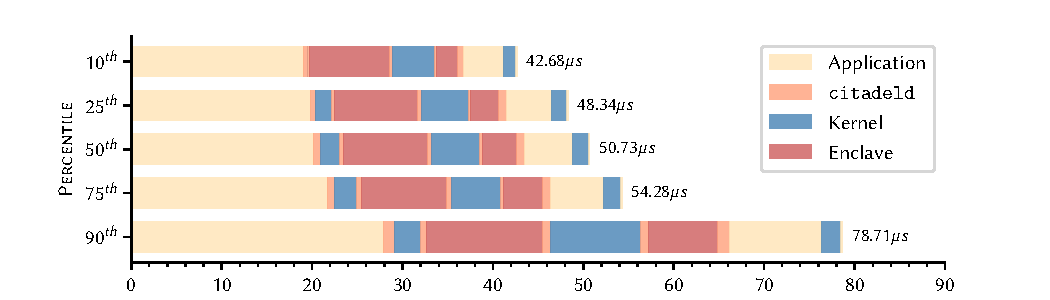
\includegraphics[width=\linewidth]{figures/graphs/open-anatomy.pdf}
    \vspace{-5mm}
    \caption{Control flow inhabitation for \texttt{libcitadel}'s \texttt{c\_open()} function, $n=100$.}
    \label{fig:open-anatomy}
\end{figure}


\begin{table}
    \centering
    \newcommand\tableTop{\rule{0pt}{3ex}}
    \newcommand\tableMid{\rule{0pt}{3ex}}
    \newcommand\tableBottom{\rule[-2ex]{0pt}{0pt}}
    \newcolumntype{N}{>{\centering\arraybackslash}m{2.5in}}
    
    \renewcommand\theadfont{\normalsize}
    \renewcommand\arraystretch{1.3}
    \begin{tabular}{l@{\hskip 0.15in} r@{\hskip 0.6in} r@{\hskip 0.35in} r@{\hskip 0.35in} r} 
        
        \toprule
        & \thead{\multirow{2}{*}{\textsc{Native}}} & \multicolumn{3}{c}{\thead{\textsc{Citadel}}} \\
        \cline{3-5}
        &  & \thead{\textit{Amortised}} & \thead{\textit{Cache Miss}} & \thead{\textit{$99^{th}$ \%ile}} \\
        % \cline{1-4}
        \midrule 
        \texttt{open()} & $1.675\pm0.076$ & $6.083\pm0.129$ & $50.133\pm1.482$ & $2.38\times$\\
        \texttt{read()} & $5.724\pm0.206$ & $7.010\pm0.192$ & $54.736\pm1.556$ & $1.26\times$\\
        \texttt{write()} & $14.340\pm0.208$ & $15.597\pm0.250$ & $63.824\pm1.902$ & $1.05\times$\\
        \texttt{close()} & $0.651\pm0.005$ & \multicolumn{2}{c}{$0.718\pm0.011$} & $1.10\times$\\

        

        \midrule 
        \texttt{socket()} & $1.446\pm0.179$ & \multicolumn{2}{c}{$3.156\pm0.291$} & $1.02\times$\\
        \texttt{bind()} & $0.762\pm0.023$ & $1.911\pm0.183$ & $49.110\pm1.746$ & $2.78\times$\\
        \texttt{listen()} & $0.705\pm0.015$ & $1.882\pm0.149$ & $48.411\pm1.386$ & $2.91\times$\\
        \texttt{connect()} & $16.570\pm0.278$ & $17.961\pm0.330$ & $66.273\pm2.147$ &$1.05\times$\\

        \midrule 
        \texttt{shmget()} & $1.880\pm0.122$ & $1.913\pm0.111$ & $49.326\pm1.466$ & $0.98\times$\\
        \texttt{shmat()} & $0.420\pm0.005$ & $1.575\pm0.134$ & $47.997\pm1.560$ & $0.99\times$\\
        \texttt{shmctl()} & $0.418\pm0.005$ & $0.743\pm0.083$ & $45.912\pm1.114$ & $0.97\times$\\
        \texttt{shmdt()} & $0.415\pm0.003$ & \multicolumn{2}{c}{$1.342\pm0.040$} & $1.01\times$\\



        \midrule 
        \texttt{pipe()} & $1.110\pm0.061$ & $1.288\pm0.069$ & $47.334\pm1.147$ & $1.02\times$\\
        \texttt{mkfifo()} & $3.865\pm0.048$ & $11.509\pm0.405$ & $59.623\pm1.788$ & $1.93\times$\\

        \midrule 
        \texttt{fork()} & $47.866\pm3.175$ & $48.647\pm3.457$ & $81.174\pm3.829$ & $15.77\times$\\
        \texttt{citadel\_init()} & $-$ & $0.801\pm0.009$ & $34.940\pm1.329$ & ---\\
        \bottomrule
    \end{tabular}
    \vspace{5mm}
    \captionsetup{justification=centering}
    \caption[\texttt{libcitadel} microbenchmarks]{\texttt{libcitadel} microbenchmarks. \\ All values are in $\mu s$ and the sample standard deviation is shown alongside the mean. For \textsc{Citadel}, both the amortised and average cache-miss durations are given. Only one value is given if the operation is not affected by a cache miss. The overhead between \textsc{Citadel} and Native Linux at the $99^{th}$ percentile is also presented. $n=10^6$.}
    \label{table:syscall-microbenchmarks}
\end{table}

\begin{figure}[h]
    \centering
    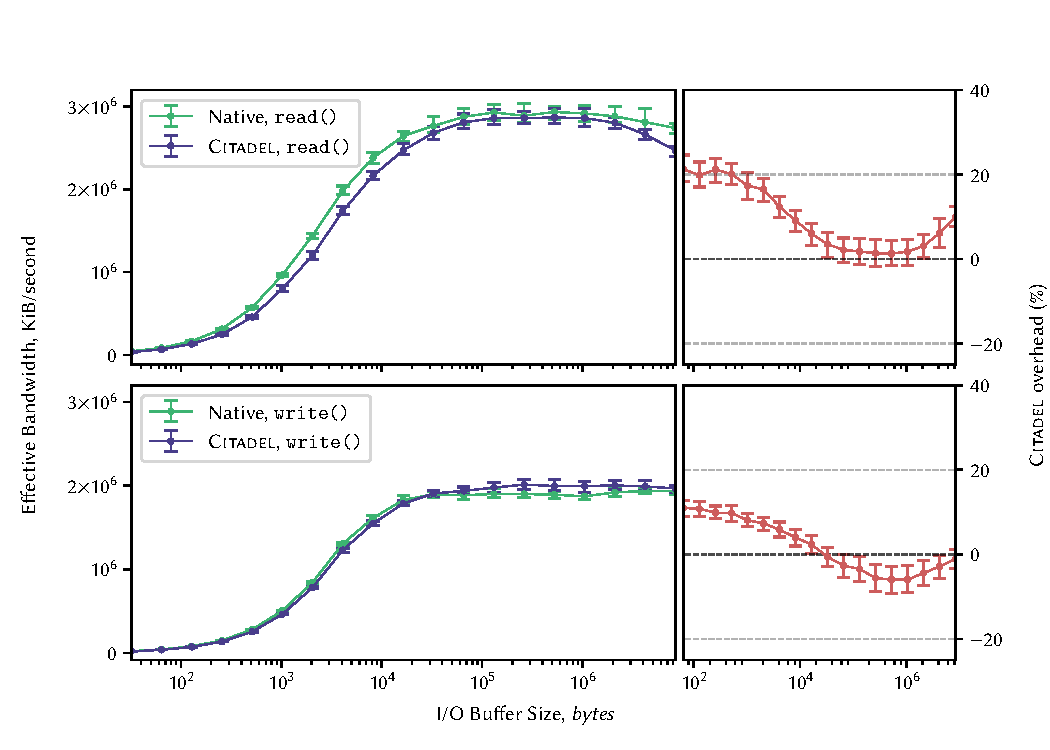
\includegraphics[width=\linewidth]{figures/graphs/io.pdf}
    \vspace{-5mm}
    \captionsetup{justification=centering}
    \caption[Effective \texttt{read()/write()} bandwidths for both the native Linux kernel and \textsc{Citadel}.]{Effective \texttt{read()/write()} bandwidths for both the native Linux kernel and \textsc{Citadel}. The percentage overhead is also presented. $n=200$ per buffer size.}
    \label{fig:io-graph}
\end{figure}

\paragraph{} A custom benchmark tool was built to assess the overall impact \textsc{Citadel} has on \textit{syscall} performance --- for example, the duration of \texttt{open()} compared to \texttt{c\_open()}. Table~\ref{table:syscall-microbenchmarks} presents these results. To give a fair comparison, two figures are reported for \textsc{Citadel}. \textit{Amortised} refers to the normal operation of \texttt{libcitadel}, in which the majority of queries are served from the cache; overhead arises from both local cache operations and added kernel latency from the \acrshort{lsm}. The other column, \textit{Cache Miss}, gives the overhead when caching is disabled, thus including communication with \texttt{citadeld}.

\paragraph{} Overall \texttt{libcitadel} contributes $\sim{}1 \mu s$ of overhead (amortised) on average --- this rises to $\sim$~$40 \mu s$ on a cache miss. Figure~\ref{fig:open-anatomy} presents a more detailed view of where exactly this overhead arises, approximately plotting where the control flow for \texttt{c\_open()} moves (on a cache miss). Interestingly, the slowest component is the communication channel between \texttt{libcitadel} and \texttt{citadeld} (median $26\mu s$);\footnote{Included in the \textit{Application} regions.} as a result, the core reference monitor functionality only adds a median penalty of $24\mu s$. The final \textit{Kernel} call before terminating is the internal call to \texttt{open()}. Additionally, the $10^{th}$ percentile demonstrates that the first \textit{Kernel} call is not always required if the entity's metadata is resident in the \texttt{citadeld} cache. During these experiments, \texttt{citadeld} showed to reliably handle over 30,000 requests/second and between $90-100\%$ usage of a single thread.

\paragraph{} Figure~\ref{fig:io-graph} plots observed effective bandwidth whilst reading from and writing to a 16 MiB file with different sized buffers; the corresponding percentage overhead inflicted by \textsc{Citadel} is plotted to the right. The benchmark driving this was adapted for Linux from one written by R.~Watson for FreeBSD.~\cite{l41-benchmark} The results clearly show \textsc{Citadel} having a more adverse effect on performance for smaller buffer sizes; unsurprising, as smaller buffers force a larger number of calls to \texttt{read()} / \texttt{write()}. It is unclear why \textsc{Citadel} provides better performance for large buffers with \texttt{write()}, an unexpected artefact --- the difference is statistically significant for buffers in the range $256$KiB and $2$ MiB, and reproducible. More work is required to determine the root causes, but hypotheses include the slight optimisation afforded by regular, small delays easing pressure on microarchitectural caches.





\subsection{IPC Microbenchmarks}
\label{sec:ipc-microbenchmarks}

\paragraph{} Again using the modified Watson benchmark, we investigated \textsc{Citadel}'s effect on end-to-end \acrshort{ipc} performance. We investigate \textit{pipes}, \textit{local sockets} (\texttt{socketpair()}), and \textit{regular sockets}, between 2 threads (Figure~\ref{fig:ipc-2thread-graph}) and between a parent and child process (Figure~\ref{fig:ipc-2proc-graph}).

\paragraph{} Overall, the results between the two contexts are similar --- both see approximately 20\% degradation in the worst cases, tending towards equal performance when using $\sim 10^5$-byte blocks. At first glance it appears that \textsc{Citadel} affects the performance between 2 threads slightly more than 2 processes, but in fact \textsc{Citadel} performs near-identically in both. Native performance is more heavily optimised when sending between two threads; \textsc{Citadel} overshadows any latency gained by the kernel.

\paragraph{} In a similar way to \texttt{write()}, \textsc{Citadel} unexpectedly outperforms the native kernel in both contexts using \texttt{pipe()}. The readings are noisy, but statistically significant for buffers in the range 16 KiB to 8 MiB, and reproducible. The cause is again unknown, but observing that the native kernel's throughput halves after buffers of 8 KiB, we suspect that this is the result of cache exhaustion or inopportune paging. Notably, \textsc{Citadel}'s readings exhibit a far larger \acrshort{iqr} for large buffer sizes than the native kernel, a side effect that is repeated in real-world testing.

\begin{figure}[]
    \centering
    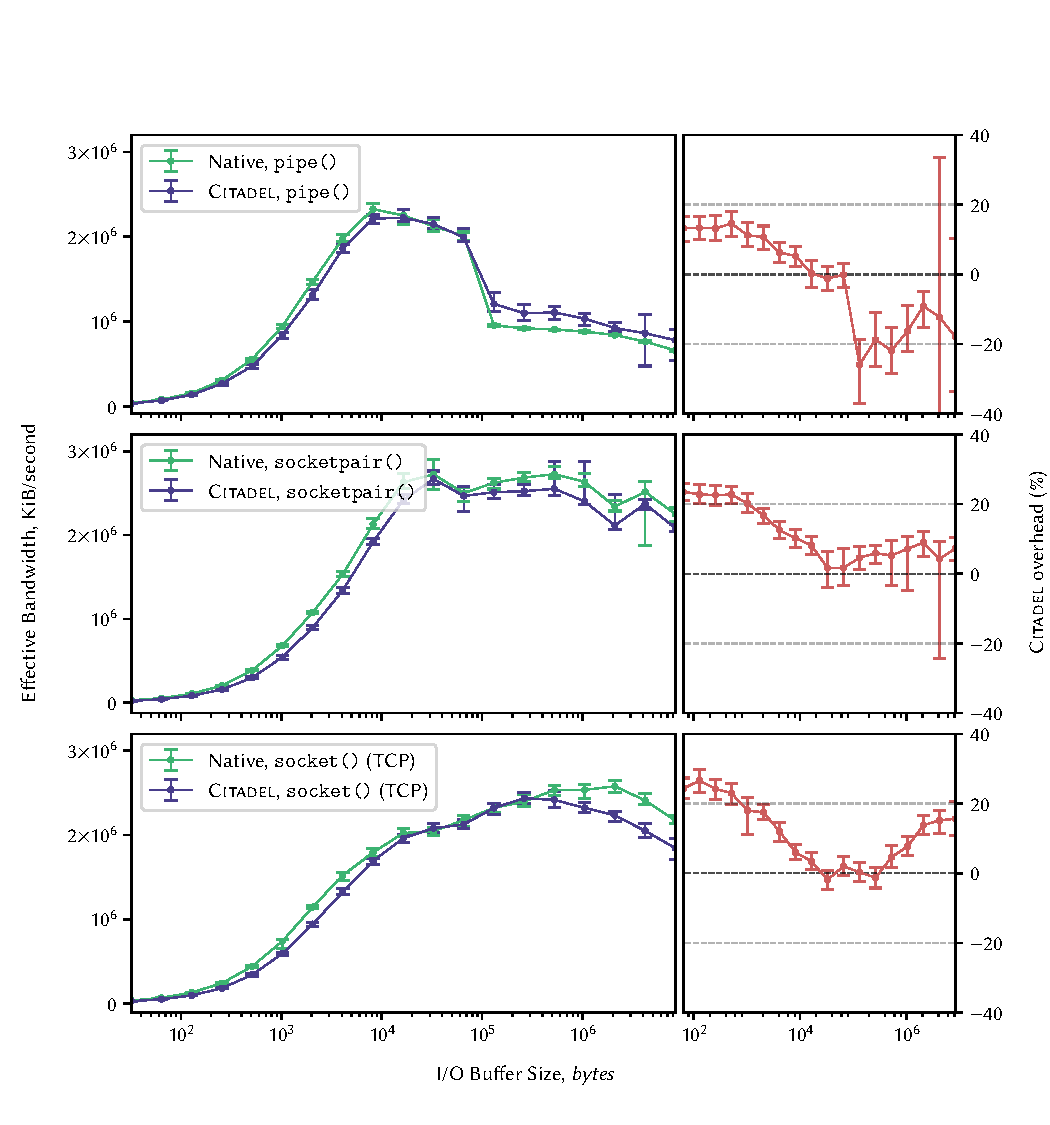
\includegraphics[width=\linewidth]{figures/graphs/ipc-2thread.pdf}
    \vspace{-5mm}
    \caption[Effective bandwidths for various types of IPC between \textit{2 threads}.]{Effective bandwidths for various types of \acrshort{ipc} between \textit{2 threads}, $n=200$.}
    \label{fig:ipc-2thread-graph}
\end{figure}


\begin{figure}[]
    \centering
    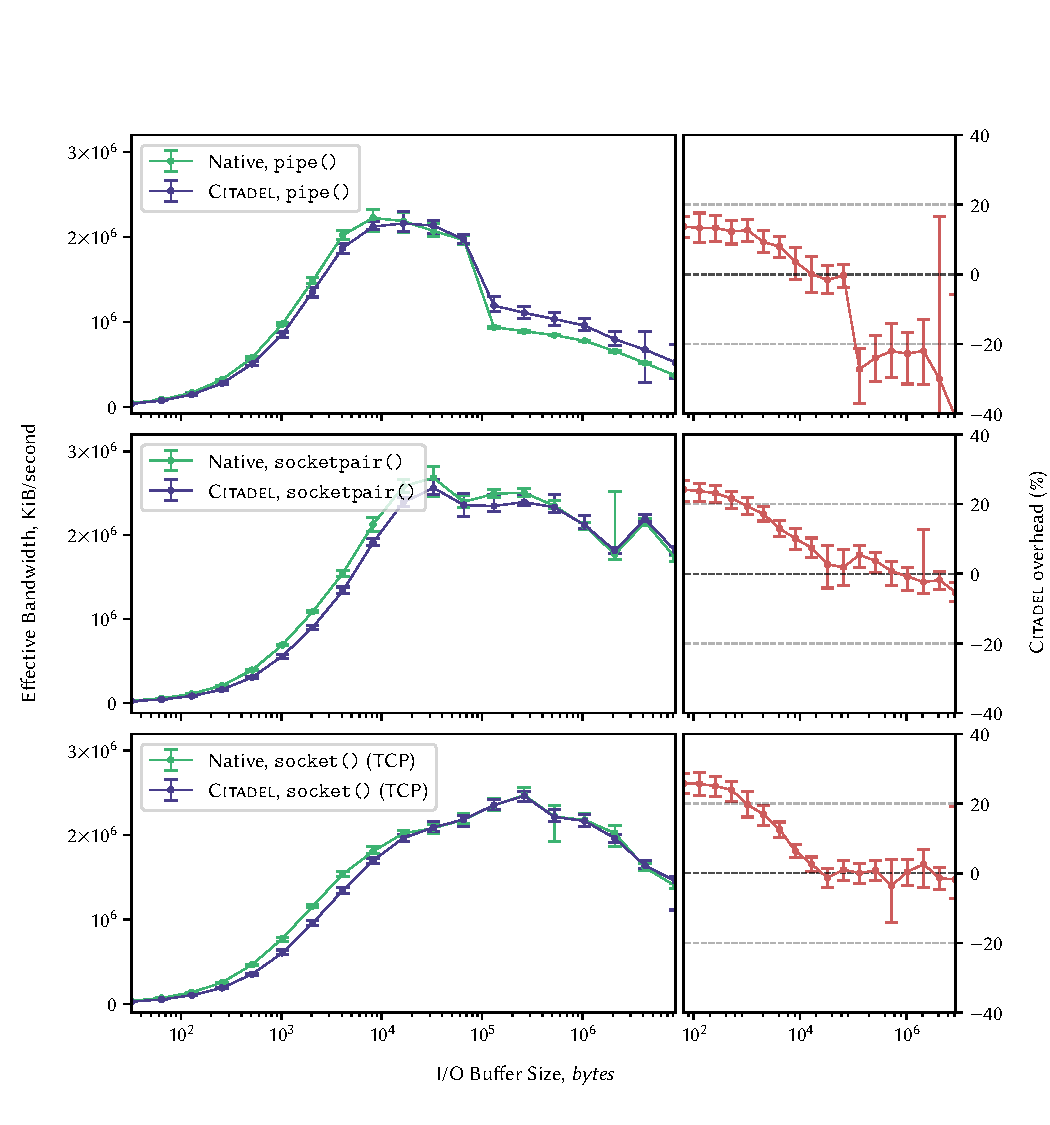
\includegraphics[width=\linewidth]{figures/graphs/ipc-2proc.pdf}
    \vspace{-5mm}
    \caption[Effective bandwidths for various types of IPC between \textit{2 processes}.]{Effective bandwidths for various types of \acrshort{ipc} between \textit{2 processes}, $n=200$.}
    \label{fig:ipc-2proc-graph}
\end{figure}

\clearpage

\subsection{\textsc{Nginx} Benchmarks}
\label{sec:nginx-benchmarks}
\begin{table}
    \centering
    \newcommand\tableTop{\rule{0pt}{3ex}}
    \newcommand\tableMid{\rule{0pt}{3ex}}
    \newcommand\tableBottom{\rule[-2ex]{0pt}{0pt}}
    \newcolumntype{N}{>{\centering\arraybackslash}m{2.5in}}
    
    \renewcommand\theadfont{\normalsize}
    \renewcommand\arraystretch{1.3}
    \begin{tabular}{l@{\hskip 0.35in} r@{\hskip 0.3in} r@{\hskip 0.35in} r@{\hskip 0.35in} c} 
        
        \toprule
        & \thead{\multirow{2}{*}{\textsc{Native}}} & \multicolumn{3}{c}{\thead{\textsc{Citadel}}} \\
        \cline{3-5}
        &  & \thead{\textit{Untainted}} & \thead{\textit{Tainted}} & \thead{\textit{Overhead}} \\
        % \cline{1-4}
        \midrule 
        \multicolumn{5}{l}{\textsc{Webserver Benchmark}, \textit{100-byte packets}} \\
        \textit{Latency} & $35.73\mu s$ & $36.18\mu s$ & $44.35\mu s$ & $24\%$ \\
        $-\;$ \textit{std. dev.} & $13.85\mu s$ & $14.12\mu s$ & $13.26\mu s$ & \\
        $-\;$ \textit{max.} & $536\mu s$ & $554\mu s$ & $508\mu s$ & \\
        \textit{Requests/s} & $2.748 \cdot 10^4$ & $2.717 \cdot 10^4$ & $2.214 \cdot 10^4$ & $19\%$\\
        \textit{Bandwidth} & $177.28$ Mbps & $168.72$ Mbps & $143.04$ Mbps & $18\%$\\

        \midrule 
        \multicolumn{5}{l}{\textsc{10GB File Transfer}} \\
        \textit{Bandwidth} & $1.404$ Gbps & $1.410$ Gbps & $1.413$ Gbps & $\sim 0\%$ \\
        $-\;$ \textit{std. dev.} & $0.428$ Gbps & $0.440$ Gbps & $0.549$ Gbps &\\
        \textit{Duration} & $56.98 s$ & $56.74 s$ & $56.62 s$ & $\sim 0\%$ \\
        $-\;$ \textit{std. dev.} & $19.45 s$ & $18.97 s$ & $23.63 s$ & \\
        
        \bottomrule
    \end{tabular}

    \vspace{5mm}
    \captionsetup{justification=centering}
    \caption{\textsc{Nginx} performance comparinson between native Linux, and both untainted and tainted \textsc{Citadel}, $n=25$.}
    \label{table:nginx-benchmarks}
\end{table}

\paragraph{} To validate the performance results presented thusfar, we ported the entirety of the \textsc{Nginx} webserver\footnote{\url{https://www.nginx.com/}} to function alongside \textsc{Citadel}. No optimisations were made to the codebase --- the only changes made replaced core \texttt{libc} function calls to use their \texttt{c\_*} \texttt{libcitadel} counterparts.

\paragraph{} Two trials were run; a low-latency benchmark\footnote{\url{https://github.com/wg/wrk}} and a 10GB \acrshort{http} file transfer (high-bandwidth). The webserver was configured to only run a single server process to ensure it was exercised to its full extent, and was set up to use the \textit{loopback} interface\footnote{\texttt{http://127.0.0.1/}.} to eliminate any interference from outside the \acrshort{os}. 

\paragraph{} The results are not surprising (Table~\ref{table:nginx-benchmarks}). For the low latency tests we observe the same $20-25$\% overhead as seen from \acrshort{tcp} sockets in §~\ref{sec:ipc-microbenchmarks} using the same buffer size. The high-bandwidth tests show \textsc{Citadel} performing equally to the native kernel, only differing by its larger sample standard deviation. This trial is also interesting as this is the first time we see file descriptor revalidation happening automatically on \texttt{read()} and \texttt{write()}. The \acrshort{cpu} overhead from \texttt{citadeld} was $<1\%$.





\section{Security}

\subsection{\textsc{Citadel} TCB}
\label{sec:citadel-tcb}

\paragraph{} One of the core initial goals of this project was to build an enclave-based reference monitor whilst \textit{minimising inflation to the system's \acrshort{tcb}}; to this end we present the trusted components of a \textsc{Citadel} system.

\begin{itemize}
    \item[---] The \acrshort{sgx} Platform, including all libraries and \textit{isgx}. 
    \item[---] The \textit{policy enclave} implementation.
    \item[---] The untrusted \texttt{citadeld} application; discussed further below.
    \item[---] The core Linux kernel, including the \textsc{Citadel} \acrshort{lsm} and the Linux \acrshort{vfs}.   
    \item[---] The Intel \textit{\acrshort{aesni}} Linux driver. 
\end{itemize}

\paragraph{} We also assume that the build environment is entirely trusted. A notable exclusion from the \acrshort{tcb} is the majority of Linux drivers and other kernel modules --- this was a strong motivation for using \acrshort{sgx}, as it can effectively defend against malicious and misbehaving ring-0 parties. 

\paragraph{} However, how might the system defend against \texttt{citadeld}, an un\-privileged, user\-space application, being replaced by a malicious adversary?

% \begin{enumerate}
%     \item How does the system defend against \texttt{citadeld}, an unprivileged, userspace application, from being replaced by a malicious adversary?
%     \item Can the kernel actually be held to the same integrity level as an enclave? Additionally, by extension, how trustable is a system that enclaves can only attest to half of?
% \end{enumerate}

\paragraph{} The compiled \texttt{citadeld} application could be protected in exactly the same way that \textsc{Citadel} defends its socket, \texttt{/run/citadel.socket}, with a reserved identifier. For example, opting to mark it with an \textit{\acrshort{xattr}} such as \texttt{security.citadel.daemon} with a \textit{nonce} value during the build process provides the \acrshort{lsm} ample confidence that an executable is a valid product of a \textsc{Citadel} build,\footnote{Using the \texttt{bprm\_check\_security} \acrshort{lsm} hook.} and protects it from tampering. This may also be valuable for defending the enclave object files themselves; although they cannot be tampered with, an adversary may try to remove them to deny service. These features would require extending the \textsc{Citadel} build system further.

\paragraph{} Secondly, can the kernel actually be held to the same integrity level as an enclave? How trustable is a system that enclaves can only attest to half of?

\paragraph{} Enclaves are unique in that their online attestation process inspires absolute trust, but offline provenance can be equally valuable. Although not \acrshort{sgx}-based, \textit{\acrshort{uefi} Secure Boot}~\cite{Richardson2013UefiSB} is an industry-standard mechanism for verifying whether an \acrshort{os} is legitimate. Ensuring that a \textsc{Citadel} system's installation is properly signed by a trusted party defends against many types of attack. 

\paragraph{} One example that \textsc{Citadel} cannot defend against has a malicious superuser compiling a new kernel with a modified \acrshort{lsm}, using valid keys scraped from the Linux system binary, and booting into it to bypass \textsc{Citadel}'s protections. Although not a bespoke solution, verifying an \acrshort{os} is well-explored and thus not a direct concern for this work. Additional protections include Linux's \textit{\acrlong{ima}} (§~\ref{sec:ima}).

\paragraph{} Thirdly, does the kernel protects itself adequately from malicious kernel modules?

\paragraph{} Effective protection is possible if carefully executed. Appendix~\ref{appendix:pid-tampering} presents a proof of concept kernel module that changes a process's \acrshort{pid} dynamically. This is highly concerning, as a process's \acrshort{pid} is its core identifier in \textsc{Citadel}'s eyes; defence was discussed in §~\ref{sec:pid-protection}. The Linux kernel is a soup of \textit{exported} and \textit{unexported symbols},\footnote{Symbols include functions and variables held in the global namespace; exporting is the process of exposing it publicly to be called by third parties.} which is exploitable to access internal functions never designed to be called from a different context. This work does not assess the implications for the \acrshort{lsm} framework, but highlights the potential need for \textit{defensive programming} when designing the \acrshort{lsm}.

\paragraph{} We believe that \textsc{Citadel}, with its restricted \acrshort{tcb}, can be trustworthy, creating a system of integrity checks based upon, and complementing, the trust placed in \acrshort{sgx} itself.

\subsection{IFC Model Implications}
\label{sec:ifc-model-implications}

\paragraph{} The \textsc{Citadel} \acrshort{ifc} model deviates from the designs and implementations of Pasquier et al. and Krohn et al. in three key ways;
\begin{enumerate}
    \item Policy and enforcement decision are separated.
    \item Passive entities may exist in a temporary \textit{transient} state.
    \item Operations between untainted entities are not mediated.
\end{enumerate}

\paragraph{} The first is handled with an extension to the core model to make policy decisions explicit and communicable (§~\ref{sec:permissible-operations}). This relationship is the core focus of this work, and \textsc{Citadel} at all points relies on conservative assumptions --- if not explicitly granted, permission is withheld. By default the system tends towards complete lockdown, a defensive measure to preserve \textit{safety} if subjected to denial of service.

\paragraph{} The second point is justified with an extension to the \textit{creation flow} rule (§~\ref{sec:permissible-operations}, (\ref{eqn:new-creation})). Transient entities are only created from a secure context, under which it automatically assumes the labelling of its parent entity. This may informally be considered an extension of the process's internal state, and held to the same restrictions. Such entities may only alter their security context (via another active entity) after being declared explicitly, leaving their transient states. 

\paragraph{} Regarding the final point --- tainting in \textsc{Citadel} assumes the worst, treating any potential infraction as cause for mediation; only the policy enclave may clear a taint. Assuming that all sensitive entities are correctly labelled, \textsc{Citadel} will protect them against anything within the system. Unlabelled entities are assumed to be in the public domain, which allows normal execution and access control to proceed until the taint boundary is crossed.

\subsection{SGX Vulnerabilities}
\label{sec:sgx-vulnerabilities}
\paragraph{} This work assume that the \acrshort{sgx} platform is itself secure; a successful attack on \acrshort{sgx} obviously compromises any protection offered by \textsc{Citadel}. A number of \acrshort{sgx} vulnerabilities have been detailed;~\cite{lipp2018meltdown, vanbulck2018foreshadow, Schwarz2019ZombieLoad, ridl, vanbulck2020lvi} these are effective and highly concerning, but mitigating them is not in the scope of this project.

\section{Use Cases}

\paragraph{} In the introduction, we laid out the motivation and goals for \textsc{Citadel}, including using it as a platform for reasoning about the relationship between an enclave and its host. Standard workflows for creating an \acrshort{sgx} application uses a library \acrshort{os}, such as \textit{SGX-LKL}~\cite{priebe2019sgxlkl} and \textit{Graphene-SGX},~\cite{203255} to create a synthetic Linux environment inside the enclave supporting the primary application --- this approach subjects the enclave to some of the same flaws and issues as the underlying \acrshort{os}. Could we reach a point where the host \acrshort{os} is trusted to hold custody of sensitive assets, instead of a trend toward pure isolation?

\paragraph{} Two hypothetical scenarios are presented --- one requiring secrecy, and one integrity --- to illustrate how \textsc{Citadel} could aid enclave-application development.

\paragraph{Scenario 1} A social-media company provides a \acrshort{gdpr} platform, through which members request an archive of their data and other assets; these may be over 10~GB. Processing and collation happen inside an enclave, and an external service authenticates requests. Must the enclave seal archives after creation, before storage, and unseal them when requested? A solution using \textsc{Citadel} may offload unencrypted archives to the custody of the host \acrshort{os}, using \acrshort{ifc}'s secrecy mechanic to prevent unauthorised release. On request, the webserver requests permission to declassify the archive from the authentication authority --- no penalty need be paid for encryption.\footnote{Disk encryption should be used for offline protection.}


\paragraph{Scenario 2} An Apache Spark application partitions input data into a large number of shards. Assuming that shard-processing is protected inside an enclave, do shards need to be cryptographically signed to verify their provenance? \textsc{Citadel} would entrust this tracking to the policy enclave, which, once attested, may be considered a part of the application's trusted components.

\paragraph{} Although \textsc{Citadel} may not be suitable for the most sensitive processing tasks --- enclaves are still vital here --- it offers a lightweight protection mechanism that could potentially be, in the interest of performance, trusted in a supporting role.


\chapter{Summary and Conclusions} 
\paragraph{} This dissertation presented \textsc{Citadel}, a modular, enclave-backed reference monitor which securely and verifiably implements \acrshort{ifc} methods in the Linux kernel. By separating policy decisions and enforcement, we demonstrated a feasible approach to deep kernel integration using Intel \acrshort{sgx}; the prototype leverages Linux's security framework to realise decisions at the lowest level of the \acrshort{os}. \textsc{Citadel} optimises for performance via an auxiliary library, which conservatively predicts a process's security context, enabling unobtrusive application integration.

\paragraph{} A full implementation of the \textsc{Nginx} webserver running on \textsc{Citadel} validates this work using real-world performance benchmarks; the most punitive trial produced a 25\% overhead, but other scenarios reported performance parity with the native Linux kernel. Verifying the methods presented here should be the next step, but an extension of \textsc{Citadel} in a distributed setting also has great potential; inter-machine attestation will likely establish an exceptional degree of trust between remote components.

\paragraph{} Further work is required before \textsc{Citadel} is fully realised and production-ready, but this project successfully demonstrates the viability and potential of a symbiotic enclave-kernel relationship, which, in the long run, may prove valuable for both.


\appendix
\singlespacing

\bibliographystyle{unsrt} 
\bibliography{references} 

\end{document}
